%&../.preamble

\endofdump

\usepackage{nicematrix}

\usetikzlibrary{external}
\tikzset{external/system call={pdflatex --shell-escape --fmt=../.preamble --halt-on-error -jobname "\image" "\endofdump\texsource"}}
\tikzexternalize[prefix=tikz/]

\title{Geometria e algebra lineare}
\author{Mattia Marini}
\date{14.09.22}

\graphicspath{{Images}}

\begin{document}

\maketitle
\tableofcontents
\listofdefs
\listoftheorems
\listofincomprensioni


\section{Vettori geometrici}
\subsubsection*{Vettore geometrico nel piano}\phantom{a}

Prendo due punti A,B. Il vettore $\vec{AB} = \left( x_B - x_A, y_B - y_A \right)  \in \R^2$

\subsubsection*{Vettore geometrico nello spazio}\phantom{a}

Prendo due punti A,B. Il vettore $\vec{AB} = \left( x_B - x_A, y_B - y_A, z_B - z_A \right)  \in \R^2$

\begin{center}
	\tcbox{NB: $\vec{{AB}} = \vec{{CD}} $ se e solo se A,B,C,D sono i vertici di un parallelogramma}
\end{center}

\subsection{Somma e prodotto per scalare}

\begin{definizione}{Somma vettori}
	Dati due vettori di componenti $\left( a_1, a_2 \right), \left( b_1,b_2 \right) $ la loro somma è definita come somma delle loro componenti:
	\[
		\left( a_1, a_2 \right), \left( b_1,b_2 \right) = \left( a_1+b_1, a_2+b_2 \right)
	\]
\end{definizione}

\begin{definizione}{Prodotto per scalare}
	Dato un vettore di componenti $\left( a_1, a_2 \right)$ e uno scalare $k$ il prodotto scalare è definito nel seguente modo:
	\[
		k\left( a_1,a_2 \right) = \left( ka_1, ka_2 \right)
	\]
\end{definizione}

La stessa cosa vale per vettori in $\R^{3}$

\subsubsection*{Interpretazione grafica somma vettori}
Graficamente la somma vettoriale si può rappresentare con la regola del parallelogramma o del punta coda:

\begin{center}
	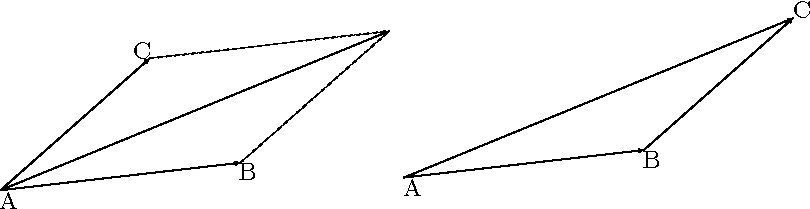
\includegraphics{Images/Somma vettori.pdf}
\end{center}

Allo stesso, il \underline{prodotto vettoriale} si può interpretare graficamente come un allungamento per un fattore $k$ di un vettore v:

\begin{center}
	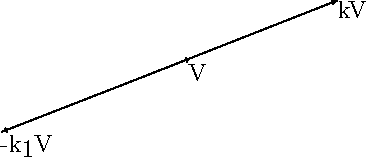
\includegraphics{Images/Prodotto per scalare.pdf}
\end{center}

\[
	\R^2 = \left\{ \left( a_1, a_2 \right) | a_1,a_{2}  \in \R \right\}
\]
\[
	\R^{3} = \left\{ \left( a_1,a_2,a_3 \right) | a_1,a_2,a_3  \in \R \right\}
\]

\begin{center}
	\tcbox{{NB: $\vec{{AB}} + \vec{BC} = \vec{AC}$ (regola del punta coda)}}
\end{center}

\subsubsection*{Proprietà somma vettori}
\label{sub:proprietàsommavettori}
\begin{itemize}
	\item Proprietà associativa \rarr è ovvio visto che la somma di numeri naturali è associativa
	\item Esistenza elemento neutro $\vec{AB} + 0 = AB$
	\item Per ogni vettore geometrico $\vec{{AB}}$ esiste un vettore simmetrico (indicato con $-AB$) che sommato ad AB risulta $\vec{0}$
	\item Proprietà commutativa
	      i
\end{itemize}

\begin{center}
	\tcbox{Posso riassumere queste proprietà affermando che $V^2$ è un \textbf{gruppo commutativo} }
\end{center}

\section{Rette e piani}
\subsection{Rette}
L'equazione di una retta può essere ricavata immaginandosi di prendere un vettore per due punti, moltiplicarlo per uno scalare variabile  $t$ e poi traslare in tutto forzando il passaggio per uno dei due punti del vettore originario. Ottengo in questo modo l'equazione parametrica:
\[
	\begin{cases}
		x = x_1 + t\left( x_2-x_1 \right) \\
		y = y_1 + t\left( y_2-y_1 \right) \\
		z = z_1 + t\left( z_2-z_1 \right)
	\end{cases}
\]
\begin{tcolorbox}
	NB: se semplifico sistema che ottengo esplicitando coordinata x y e z eliminando t ottengo l'equazione di due piani la cui intersezione e la retta
\end{tcolorbox}

\subsection{Piani}
L'equazione di un piano può essere ricavata immaginandosi di prendere due vettori, allineare il punto di applicazione (metterli culo a culo), ed eseguire la combinazione lineare di questi ( $sv_1 + sv_2$) in modo da ottenere il luogo dei punti definito da un piano. Ottengo la seguente equazione parametrica:
\[
	\begin{cases}
		x = x_1 + s\left( x_2 - x_1 \right) + t\left( x_3-x_1 \right) \\
		y = y_1 + s\left( y_2-y_1 \right) + t\left( y_3-y_1 \right)   \\
		z = z_1 + s\left( z_2-z_1 \right)  + t \left( z_3-z_1 \right)
	\end{cases}
\]
Eliminando la $s$ e la $t$ posso ottenere la forma cartesiana, ad esempio:
\[
	2x - y + 5z - 4 =0
\]
\begin{center}
	\tcbox{NB: il vettore di coordinate $2,-1,5$ definize la direzione perpendicolare al piano}
\end{center}

\subsection{Lunghezza del vettore}
\label{sec:lunghezzadelvettore}
La lughezza di un vettore $\vec{v}$ viene indicata con $\left|\vec{{v}} \right|$. Noi scegliamo un sistema di riferimento con gli assi ortogonali per poter applicare il teorema di pitagora e poter evitare l'uso di seni e coseni

\[
	\left|\vec{v}\right|=\sqrt{V_x^2 + V_y^2} \text{ in } V^2 \quad \quad \left|\vec{c}\right| = \sqrt{V_x ^2 + V_y ^2 + V_z ^2} \text{ in } V^3
\]
\section{Prodotto scalare e vettoriale}
Premessa:
Siano $\vec{V} e \vec{W}$ vettori geometrici non nulli nel piano o nello spazio. Noi consideriamo l'angolo convesso ossia quelli compreso fra $\left[ 0,180 \right] $ gradi
\subsection{Prodotto scalare}
Dimostro la seguente equivalenza:
\[
	\text{ Prodotto scalare }= v_1 w_1 + v_2 w_2 + v_3w_3 =	\left|v\right|\left|w\right|\cos \theta
\]
Prendo due vettori $ \vec{W}, \vec{V}$, li metto culo a culo ed esprimo la lunghezza del terzo vettore che li congiunge:
\begin{center}
	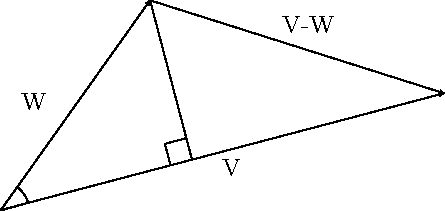
\includegraphics{Images/Prodotto scalare.pdf}
\end{center}
Condidero i due vettori $ \vec{V} \text{ e } \vec{W}  $ ed esprimo la loro differnza tramite due modi: teorema di pitagora e trigonometria
\begin{itemize}
	\item \underline{Modo 1: teorema di pitagora}
	      \[
		      \left| v-w\right| ^2 = \left( v_1-w_1 \right) ^2 + \left( v_2-w_2 \right) ^2 + \left( v_3-w_3 \right) ^2= \left|v\right|^2 + \left|w\right|^2 - 2\left( v_1w_1 + v_2w_2 + v_3 w_3\right)
	      \]
	\item \underline{Modo 2: trigonometria}
	      \[
		      \left|v-w\right|^2 = \left( \left|w\right| \sin \theta  \right) ^2 + \left( \left|v\right|- \left|w\right| \cos \omega  \right) ^2 = \left|v\right|^2 + \left|w\right|^2 - 2 \left|v\right|\left|w\right|\cos \theta
	      \]
	\item Ottengo per questo l'uguaglianza
	      \[
		      v_1w_1 + v_2w_2 + v_3 w_3 = \left|v\right| + \left|w\right| \cos \theta
	      \]
	\item Girando la formula e tenendo conto che a sinistra ho per definizione il prodotto scalare di $v$ e $w$ ottengo la seguente relazione:
	      \[
		      w \cdot v = \left|v\right|\left|w\right|\cos \theta
	      \]
\end{itemize}
\subsection{Proprietà prodotto scalare}
\begin{itemize}
	\item Bilineare:
	      \[
		      \left( \vec{u} + \vec{v} \right) \cdot \vec{w} = \vec{u} \cdot \vec{w} + \vec{v} \cdot \vec{w}
	      \]
	      \[
		      k\left( \vec{v}\cdot\vec{w} \right) = \left( k\vec{v} \right) \cdot\vec{w} = \vec{v}\cdot \left( k\vec{w} \right) \quad \forall k \in  \R
	      \]
\end{itemize}

\subsection{Significato coefficienti in equazione cartesiana retta e piano}
In una retta $r$ con equazione cartesiana $ax + by = c$ i coefficienti $a $ e $b$ costituiscono \underline{un vettore ortogonale alla retta $r$}
\begin{itemize}
	\item Prendo $P_1 \left( x_1,y_2 \right) $ e $P_2 \left( x_2,y_2 \right) $ in modo tale che appartengano alla retta:
	      \[
		      ax_1 + by_1 = c \quad ax_2+ by_2= c
	      \]
	\item Mettendo a sistema le due relazioni ottenute e sottraendole ottengo che:
	      \[
		      a\left( x_2-x_1 \right) + b\left( y_2-y_1 \right)  = 0
	      \]
	\item Noto che ciò che ho ottenuto a sinista è il \underline{prodotto scalare del vettore di coordinate  $\left( a,b \right) $ e $\vec{P_1P_2}$}; per questo $\left( a,b \right) $ definisce un vettore \underline{ortogonale alla retta}
\end{itemize}
Eseguento il medesimo ragionamento posso affermare che in un piano $\pi$ con equazione $ax + by + cz +d =0$ il vettore di coordinate $\left( a,b,c \right) $ sia ortogonale al piano $\pi$

\subsection{Prodotto vettoriale}
Il prodotto vettoriale fra due vettori $\vec{v}$ e $\vec{w}$ è uguale all'area del parallelogramma definito da questi ultimi. Posso dimostrare abbastanza facilmente il suo valore:
\begin{align*}
	A^2= \left|\vec{v}\right|^2\left|\vec{w}\right|^2 \sin ^2\theta & = \left|\vec{v}\right|^2\left|\vec{w}\right|^2 \left( 1- \cos^2 \theta   \right)                \\
	                                                                & = \left( v_1^2 + v_2^2 \right) \left( w_1^2 + w_2^2 \right) - \left( v_1w_1 + v_2w_2 \right) ^2 \\
	                                                                & = \left( v_{1}w_2- v_{2}w_1 \right) ^2
\end{align*}
Posso definire quindi il prodotto vettoriale:
\begin{definizione}{Prodotto vettoriale}
	Il prodotto scalare fra due vettori $\vec{v}$ e $\vec{w}$ è uguale all'area del paralelogramma definito da questi ultimi e si può esprimere nel seguente modo:
	\[
		\vec{v} \times \vec{w} = \left|v\right|\left|w\right| \sin \theta = \left( v_2w_3 - v_3w_2, v_3w_1-v_1w_3, v_1w_2-v_2w_1 \right)
	\]
\end{definizione}

\begin{itemize}
	\item $\vec{w} \times \vec{v} = - \vec{v} \times \vec{w}$
	\item Il prodotto è nullo se e solo se i vettori sono paralleli o proporzionali
	\item La direzione di $ \vec{v} \times \vec{w}$ è ortogonale a $\vec{v}, \vec{w}$
	\item Il verso del vettore prodotto vettoriale si determina con la regola della mano destra
	\item La quantità $ \left( \vec{v} \times \vec{w} \right) \cdot \vec{u} $ è l'area del parallelepipedo di lati $\vec{u},\vec{v},\vec{w}$
\end{itemize}


\section{Gruppi}
\begin{definizione}{Gruppo}Un gruppo è un insieme $G$ su cui è definita un'operazione $*$  \[
		* : G \times G \rightarrow G
	\]
	Tale operazione deve soddisfare 3 specifiche:
	\begin{itemize}
		\item E' associativa $ \left( a*b \right) *c = a* \left( b*c \right) $
		\item Esiste l'elemento neutro $ \exists e  \in G \text{ t.c. }e* a = a * e = a$
		\item $ \forall a  \in  G \quad$ esiste il simmetrico $ a'  \in G$ tale che: $ a * a' = a' * a=e$
	\end{itemize}
	Inoltre, il gruppo si dice \textbf{ commutativo} se:  \[
		a * b = b * a \quad \forall a, b  \in  G
	\]
\end{definizione}

\subsection{Esempi}
\label{sub:esempi}
\begin{itemize}
	\item $\left( \N, + \right) $ \rarr non è gruppo in quanto:
	      \begin{itemize}
		      \item è associativo
		      \item Esiste elemento neutro
		      \item Non esiste simmetrico
	      \end{itemize}
	      \item$ (\Z, +)$ \rarr è gruppo in quanto
	      \begin{itemize}
		      \item è associativo
		      \item esiste elemento neutro
		      \item Esiste simmetrico
	      \end{itemize}
	\item $ \left( \N, \times \right) $ \rarr non è gruppo (non esiste simmetrico)
	\item $\left( \Z, \times \right) $ \rarr non è gruppo (non esiste simmetrico)
	\item $ \left( \Q, \times \right) $ \rarr non è gruppo (solo per quanto riguarda lo zero $0 \cdot \text{ qualsiasi numero  }=0$)
	\item $\left( Q^* = Q \setminus \left\{ 0 \right\}, \times \right) $ \rarr è gruppo commutativo (i razionali meno lo zero)
	\item $\left( R^* = R \setminus \left\{ 0 \right\}, \times \right) $ \rarr è gruppo commutativo (i razionali meno lo zero)
	\item $\left( C^* = C \setminus \left\{ 0 \right\}, \times \right) $ \rarr è gruppo commutativo (i razionali meno lo zero)
\end{itemize}

\begin{tcolorbox}
	$K =  \Q, \R , \C$ sono detti \textbf{campi} nei quali vale la proprietà distributiva: \[
		a\left( b+c \right) = ab + ac \quad \forall a,b,c  \in K
	\]
\end{tcolorbox}

\begin{definizione}{Campi}
	Un campo è un insieme $ \mathbb{K} $ su cui sono definite due operazioni $ + $ e $\times$ tali che :
	\begin{itemize}
		\item $\left( \mathbb{K}, + \right) $ è un gruppo commutativo
		\item $ \mathbb{K} ^{*} = K \setminus \left\{ 0 \right\} , \left( \mathbb{K} ^{*}, \times \right) $ è un gruppo commutativo
		\item Vale la proprietà distributiva: $ a \times \left( b+c \right) = a \times b + a\times c \quad \forall a,b,c \in  \mathbb{k}$
	\end{itemize}
\end{definizione}

\section{n-uple}
\[
	\R ^{n}= \left\{ a= \left( a_1, \ldots, a_n \right) | a_i  \in \R, i=1, \ldots , n \right\}
\]
\subsubsection*{Addizione}
\[
	a,b  \in  \R ^{n} \quad a+b = \left( a_1 + b_1 , \ldots a_n + b_n \right)
\]
\subsubsection*{Moltiplicazione}
\[
	a  \in  \R ^{n}, k  \in  \R \quad ka= \left( ka_1, \ldots, ka_n \right)
\]
NB: è gruppo commutativo in quanto l'addizione e il prodotto sono definite come addizione e prodotto di numeri reali

\section{Matrici}

\begin{definizione}{Matrice}
	Una matrice A del tipo $m \times n$ è una tabella di m file e n colonne
	\[
		\begin{bmatrix}
			a_{11} & \ldots & a_{1n} \\
			a_{21} & \ldots & a_{2n} \\
			a_{m1} & \ldots & a_{mn}
		\end{bmatrix}
	\]
\end{definizione}
Una matrice si può scrivere in versione compatta
\[
	A= \begin{bmatrix} a_{ij} \end{bmatrix}
\]
Se $m=1$ la matrice si può identificare come una n-upla:
\[
	\begin{bmatrix}
		a_{11} & \ldots & a_{1n}
	\end{bmatrix}
	=
	\left( 	a_{11},  \ldots, a_{1n} \right)
\]
Se $ n=1$ la matrice si può identificare come una u-upla
\[
	\begin{bmatrix}
		a_{11} \\ \vdots \\ a_{m1}
	\end{bmatrix}
	=
	\left( 	a_{11},  \ldots, a_{m1} \right)
\]
Con il simbolo $M_{m,n}\left( \R \right) $ si indica l'insieme contenente tutte le matrici reali

\subsubsection*{Somma}
\label{ssub:somma}
$A,B$ di tipo $m \times n$ , $ a = \left[ a_{ij} \right] , b= \left[ b_{ij} \right] $
\[
	A + B = \left[ a_{ij}+ b_{ij} \right]
\]
\subsubsection*{Moltiplicazione}
$A$ di tipo $m \times n$ , $ a = \left[ a_{ij} \right] , k  \in  R$
\[
	kA = \left[ ka_{ij}\right]
\]
\subsection{Prodotto matriciale}
Considera $ A \quad  m \times n$ e $B \quad  n \times r$ ossia \textbf{matrici conformabili}
\vskip3mm
La matrice prodotto matriciale $ C = AB \quad m \times r$
\[
	A \quad m \times n= \begin{bmatrix}
		a_{11} & a_{12} & a_{13} \\
		a_{21} & a_{22} & a_{23} \\
	\end{bmatrix}
	\quad
	B \quad  m \times r = \begin{bmatrix}
		b_{11} & b_{12} \\
		b_{21} & b_{22} \\
		b_{31} & b_{32}
	\end{bmatrix}
\]
\[
	AB= \begin{bmatrix}
		\left( a_{11}  b_{11} \right) + \left( a_{12} b_{21} \right) + \left( a_{13} b_{31} \right) & \left( a_{11} b_{12} \right) + \left( a_{12} b_{22} \right)  + \left( a_{13} b_{32} \right) \\
		\left( a_{21} b_{11} \right) + \left( a_{22} b_{21} \right) + \left( a_{23} b_{31} \right)  & \left( a_{21}b_{12} \right) + \left( a_{22}b_{22} \right) + \left( a_{23}b_{32} \right)
	\end{bmatrix}
\]
Esempio:
\[
	A = \begin{bmatrix}
		1 & 2 & 3 \\
		4 & 5 & 6 \\
	\end{bmatrix}
	\quad
	B=
	\begin{bmatrix}
		1 & 2 \\
		3 & 4 \\
		5 & 6
	\end{bmatrix}
\]
\[
	AB= \begin{bmatrix}
		22 & 28 \\
		49 & 64 \\
	\end{bmatrix}
\]
\subsubsection*{Motivazioni prodotto matriciale in sistemi lineari}
\[
	\begin{cases}
		x_1 + x_2 + x_3 = 4     \\
		2x_1 + 2x_2 + 5x_3 = 11 \\
		4x_1 + 6x_2 + 8x_3 = 24
	\end{cases}
\]

\begin{center}
	\tcbox{Questo è un sistema lineare in quanto non comapiono cose tipo $ x^2$ o $ \ln \left( x \right) $}
\end{center}

\begin{tcolorbox}
	Posso rappresentare sistema tramite matrice di coefficienti:
	\[ A=
		\begin{bmatrix}
			1 & 1 & 1 \\
			2 & 2 & 5 \\
			4 & 6 & 8
		\end{bmatrix}
		\quad
		b = \begin{bmatrix} 4 \\ 11 \\ 24 \end{bmatrix} \quad x= \begin{bmatrix} x_1 \\ x_2 \\ x_3 \end{bmatrix}
	\]
	\[
		Ax = b
	\]

\end{tcolorbox}

\subsection{Proprietà}
\begin{itemize}
	\item Il prodotto per scalare è associativo
	      \[
		      \left( k_1k_2 \right) A = k_1\left( k_2A \right) \quad
	      \]
	      e distributivo
	      \[
		      k \left( A + B  \right) = kA + kB \quad
		      \left( k_1 + k_2 \right) A = k_1 A + k_2 A
	      \]
	\item Il prodotto matriciale è associativo:
	      \[
		      \left( AB \right) C = A \left( BC \right)
	      \]
	      \[
		      k \left( AB  \right) = \left( k A  \right) B = A \left( kB \right)
	      \]
	      e distributivo rispetto alla somma:
	      \[
		      A \left( B+C \right)  = AB + AC \quad \left( A+B \right) C = AC + BC
	      \]
	      sempre che le matrici siano  \underline{conformabili}
	\item Il prodotto matriciale \underline{non} è commutativo:
	      \[
		      AB \neq BA
	      \]
	      ad esempio:
	      $$
		      \left[\begin{array}{ll}
				      1 & 0 \\
				      1 & 0
			      \end{array}\right]\left[\begin{array}{ll}
				      0 & 1 \\
				      0 & 1
			      \end{array}\right]=\left[\begin{array}{ll}
				      0 & 1 \\
				      0 & 1
			      \end{array}\right] \text { ma }\left[\begin{array}{ll}
				      0 & 1 \\
				      0 & 1
			      \end{array}\right]\left[\begin{array}{ll}
				      1 & 0 \\
				      1 & 0
			      \end{array}\right]=\left[\begin{array}{ll}
				      1 & 0 \\
				      1 & 0
			      \end{array}\right]
	      $$
	\item La matrice identica di ordine $n$ si indica con $I_n$ ed è la matrice quadrata:
	      i
	      $$
		      I_n=\left[\begin{array}{cccc}
				      1      & 0      & \cdots & 0      \\
				      0      & 1      & \cdots & 0      \\
				      \vdots & \vdots & \ddots & \vdots \\
				      0      & 0      & \cdots & 1
			      \end{array}\right]
	      $$
	      La matrice è tutta uguale a zero a parte lungo la diagonale: $I_n=\left[\delta_{i j}\right]$, con $\delta_{i j}=0$ per $i \neq j, \delta_{i j}=1$ per $i=j$. Se $A$ è una matrice conformabile con $I_n$, a destra o a sinistra, si ha $A I_n=A$ (oppure $I_n A=A$ ).
\end{itemize}

\begin{definizione}{Matrici invertibili}Sia $ A  \in  M_n \left( \R \right) $ si dice \underline{ invertibile}  se $ \exists B  \in  M_n \left( \R \right)  \text{ t.c. }$ \[
		AB = BA = I_n
	\]
	Se esiste, B \underline{è unica} e viene detta \underline{matrice inversa} di A e viene definita con $ A ^{ -1}$\end{definizione}
OSS. Il prodotto di matrici invertibili è invertibile
\[
	\left( AB \right) \left( B^{-1}A^{-1} \right) = A \left( B B ^{-1}  \right) A^{-1} = A I_n A^{-1} = A A ^{-1} = I_n
\]
Le matrici invertibili formano un gruppo in quanto:
\[
	g = \left\{ A  \in  M_{m,n} (\R) | A \text{ invertibile } \right\}
\]
\begin{itemize}
	\item $ \left( G, \times \right) $ è un gruppo (non commutativo)
	      \begin{itemize}
		      \item E' associativa in quanto anche $ M_{m,n} (\R)$ è associativa
		      \item Matrice neutra è presente
		      \item Ogni matrice ha il suo simmetrico (radice inversa)
	      \end{itemize}
\end{itemize}
\begin{definizione}{Potenze}Sia $A$ una radice $m \times n$ la \underline{potenza k-esima } di A è la radice
	\[
		A^{k} = \underbrace{A \cdot A \cdot A \ldots A}_{\text{k volte}}
	\] \end{definizione}
NB: \[
	A^{i}A^{j} = A^{i+j} = A^{j}A^{i}
\]
\begin{definizione}{Matrice trasposta}
	Si dice \underline{matrice trasposta} di $A \quad m \times n$ e si indica con $ A ^{ T}$ la matrice \[
		A^{T}= \left[ a_{ji} \right] \quad n \times m
	\]
	ossia inverto righe e colonne
\end{definizione}
OSS: \[
	\left( AB \right) ^{T} = B ^{T}A^{T}
\]
\begin{definizione}{Matrice simmetrica}
	Se $A = A^{T} \rightarrow n = m$ A è detta simmetrica, ossia è speculare rispetto alla diagonale
\end{definizione}
\section{Sistemi e matrici}
\label{sec:sistemiematrici}

Dato il sistema
\[
	\begin{cases}
		x_1 + x_2 + x_3 = 4     \\
		2x_1 + 2x_2 + 5x_3 = 11 \\
		4x_1 + 6x_2 + 8x_3 = 24
	\end{cases}
\]
\[
	x_1 \begin{bmatrix} 1\\1\\3 \end{bmatrix}  + x_2 \begin{bmatrix} 1\\2\\6 \end{bmatrix} + x_3\begin{bmatrix} 1\\5\\8 \end{bmatrix} = \begin{bmatrix} 4\\11\\24 \end{bmatrix}= b
\]
OSS: il sistema è risolubile se e solo se il vettore b è combinazione lineare delle colonne di A
\begin{definizione}{Combinazione lineare per matrici}
	Date $A_1, \ldots , A_k$ matrici $m\times n$ e dati k scalari $c_1, .., c_k  \in  \R$ la \underline{ combinazione lineare }di $A_1, \ldots , A_k$ con $c_1, .., c_k$ è la matrice \[
		c_1A_1 + c_2 A_2 \ldots + c_k A_k \quad  m\times n
	\]
\end{definizione}

\subsection{Matrici e grafi}

\begin{definizione}{Matrice di adiacenza}
	Dato un grafo $ \left( V, E \right) $ la sua \underline{ matrice di adiacenza} A è la matrice $ m\times n $ (n numero di vertici) con elemto $a_{ij}=$ numero di lati dal vertice $V_i$ al vertice $V_j$
\end{definizione}

\begin{teorema}{Numero cammini in grafo}
	L'elemento di posto $ \left( i, j  \right) $ nella matrice $ A ^{ S}$ è il numero di \underline{cammini di lungheza S} che iniziano in $ V_i $ e terminano in $ V_j$
\end{teorema}
Spiegazione:
\begin{itemize}
	\item Penso a caso base in cui $S=2$ e faccio prodotto matriciale
	      \[
		      A=
		      \begin{bmatrix}
			      1 & 1 & 0 \\
			      0 & 0 & 2 \\
			      0 & 0 & 0 \\
		      \end{bmatrix}
		      \quad
		      A^{2} = \begin{bmatrix}
			      1 & 1 & 2 \\
			      0 & 0 & 0 \\
			      0 & 0 & 0
		      \end{bmatrix}
		      \quad A ^{3} =
		      \begin{bmatrix}
			      1 & 1 & 2 \\
			      0 & 0 & 0 \\
			      0 & 0 & 0
		      \end{bmatrix}
	      \]

	\item Provo ad esempio a trovare numero percorsi da $V_1$ a $V_3$
	\item In questo caso devo moltiplicare la riga 1 di A e la colonna 3 sempre di A: \[
	      \]

	      \[
		      \underbrace{\begin{bNiceMatrix}[margin=1pt]
				      \CodeBefore
				      \rowcolor{gray!20}{1}
				      \Body
				      1 & 1 & 0 \\
				      0 & 0 & 2 \\
				      0 & 0 & 0 \\
			      \end{bNiceMatrix}}_{\text{Frecce che partono da } V_1}
		      \underbrace{\begin{bNiceMatrix}[margin=1pt]
				      \CodeBefore
				      \columncolor{gray!20}{3}
				      \Body
				      1 & 1 & 0 \\
				      0 & 0 & 2 \\
				      0 & 0 & 0 \\
			      \end{bNiceMatrix}}_{\text{Frecce che arrivano in }V_3}
		      \rightarrow
		      \begin{bmatrix}  1 \\ 1 \\ 0 \end{bmatrix} \cdot \begin{bmatrix} 0 \\ 2 \\ 0 \end{bmatrix} = \begin{bmatrix} 2 \end{bmatrix}
	      \]
	\item Il numero di percorsi $V_1 \rightarrow V_k \rightarrow V_3$ sono dati da \[
		      V_{11} V_{13} + V_{12} V_{23} + V_{13}V_{33}
	      \]
	      ossia da prodotto matriciale che genera la cella $a_{ij}$
	      \hr
	\item A questo punto so che $A^{2}$ è una matrice che in ogni cella $a_{ij}$ contiene il \underline{numero di strade di lunghezza 2 per arrivare da $V_i a V_j$ }
	\item Effettuando il prodotto matriciale per $A$ ancora una volta eseguo una \underline{procedura ricorsiva}
\end{itemize}

\begin{definizione}{prodotto scalare n-uple}
	Il \underline{prodotto scalare} di due n-uple $x,y  \in  \R^{n}$ è il \underline{numero reale} è uguale a: \[
		x \cdot y = \sum_{k=1}^{n} x_iy_i
	\]
\end{definizione}

Proprietà:
\begin{itemize}
	\item Simmetrico \quad $x\cdot y = y \cdot x$
	\item Bilineare
	      \begin{itemize}
		      \item $(x+y)z = x \cdot z + y \cdot z$
		      \item $\left( \alpha x  \right) \cdot y = \alpha \left( x \cdot y \right) $
		      \item $x \cdot \left(  y + z \right)  = x \cdot y + x \cdot z$
		      \item $x \cdot \left( \alpha y  \right) = \alpha \cdot \left( x \cdot y \right) $
	      \end{itemize}
	\item Positivo \quad $ x \cdot x \ge 0$
\end{itemize}

\begin{definizione}{Norma di n-ulpa}
	La lunghezza \underline{ o norma} di una n-upla $ x  \in \R ^{n}$ è \[
		\|x\|= \sqrt{x \cdot x} \ge 0
	\]
\end{definizione}

\begin{definizione}{Distanza fra n-uple}
	La distanza fra $x$ e $y$ in $ \R ^{n}$ è \[
		d\left( x, y  \right) = \left|\left|x-y\right|\right|
	\]
\end{definizione}

OSS: ogni nupla può essere normalizzata, facendola diventare un versore: \[
	x' = \frac{x}{\left|\left|x\right|\right|}
\]
\begin{definizione}{Ortogonalità n-uple}
	Due n-uple $ x, y  \in  R^{ n}$ si dicono \underline{ortogonali} se $ x \cdot y =0$
\end{definizione}
Osservando la seguente figura cerco di ricavare la lunghezza di $cy$
\begin{figure}[H]
	\centering
	\input{Images/Proiezione ortogonale.pdf_tex}
	\caption{Proiezione ortogonale di un vettore}
\end{figure}

\begin{definizione}{Proiezione ortogonale}
	La proiezione ortogonale del segmento $x$ su $y$ è:
	\[
		pr_y\left( x \right) = \frac{x \cdot y}{\|y\|^2} y
	\]
\end{definizione}

\subsection{Disuguaglianza di Cauchy- Schwarz}
\[
	\forall x, y  \in  \R ^{n} \quad \left|x \cdot y \right| \le \|x\| \| y\|
\]
\textbf{Dimostrazione}
\begin{figure}[h]
	\centering
	\input{Images/Proiezione ortogonale.pdf_tex}
	\caption{Proiezione ortogonale}
\end{figure}

Per Cauchy-Schwarz, se $ x, y  \in  \R ^{ n} \quad  x \neq 0 , y \neq 0$
\[
	\left|\frac{x \cdot y}{\|x\|\| y\|}\right|  \in  \left[ 0,1 \right]
\]
\begin{definizione}{Angolo}
	Angolo convesso tra x e $ y$ (non nulli in $\R ^{n}$ ) è \[
		\theta  \in  \left[ 0 , \pi \right] \rightarrow \cos\left( \theta  \right) = \frac{x \cdot y}{\|x\| \| y\|}
	\]
\end{definizione}

\subsection{Distanza tra rette sghembe}
OSS: Fra due rette sghembe esiste un \underline{solo segmento} che sia ortogonale a entrambe le rette. La lunghezza di tale segmento costituisce la distanza fra le due rette
\begin{itemize}
	\item Prendo generico punto $P$ sulla retta $r$ e un punto generico $Q$ sulla retta $r'$
	\item Scrivo lunghezza vettore $\vec{PQ}$
	\item Impongo che il prodotto scalare fra $\vec{PQ} $, $ \vec{V_r}$ e $\vec{V_{r'}}$ sia 0: \[
		      \begin{cases}
			      \vec{PQ} \cdot \vec{V_r} =0 \\
			      \vec{PQ} \cdot \vec{V{r'}} = 0
		      \end{cases}
	      \]
	\item Risolvendo il sistema trovo i valori in corrispondenza dei quali il segmento $\vec{PQ}$ è \underline{ortogonale a entrambe le rette.} Calcolo lunghezza del segmento in corrispondenza dei valori trovati
\end{itemize}

\section{Metodo di eliminazione di Gauss Jordan}
Operazioni disponibili in una matrice
\begin{itemize}
	\item $S_{ij}$ - scambio righe
	\item $D_i\left( c \right) $ - moltiplico riga per scalare $ c $
	\item $E_{ij}\left( c \right) $ - somma di riga $ i$ con $j$ moltiplicata per uno scalare $ c $
\end{itemize}
\subsection{Sistema risolvibile}

\[
	\begin{bmatrix}
		1 & 1 & 1 & 4  \\
		2 & 2 & 5 & 11 \\
		4 & 6 & 8 & 24
	\end{bmatrix}
	\rightarrow
	E_{21}\left( -2 \right) , E_{31}\left( -4 \right)
	\rightarrow
	\begin{bmatrix}
		1 & 1 & 1 & 4 \\
		0 & 0 & 3 & 3 \\
		0 & 2 & 4 & 8
	\end{bmatrix}
	\rightarrow
	S_{23}
	\rightarrow
	\begin{bmatrix}
		1 & 1 & 1 & 4 \\
		0 & 2 & 4 & 8 \\
		0 & 0 & 3 & 3
	\end{bmatrix}
\]
posso semplificare ulteriormente, ad esempio rendo coefficienti $x_1, x_2, x_3$ uno
\[
	D_2\left( \frac{1}{2} \right) , D_3\left( \frac{1}{3} \right) \rightarrow
	\begin{bmatrix}
		1 & 1 & 1 & 4 \\
		0 & 1 & 2 & 4 \\
		0 & 0 & 1 & 1
	\end{bmatrix}
	\rightarrow
	E_{23}\left( -2 \right) \rightarrow
	\begin{bmatrix}
		1 & 1 & 1 & 4 \\
		0 & 1 & 0 & 2 \\
		0 & 0 & 1 & 1
	\end{bmatrix}
\]
\[
	\rightarrow
	E_{12}\left( -1 \right) \rightarrow
	\begin{bmatrix}
		1 & 0 & 1 & 2 \\
		0 & 1 & 0 & 2 \\
		0 & 0 & 1 & 1
	\end{bmatrix}
	E_{13}\left( -1 \right) \rightarrow
	\begin{bmatrix}
		1 & 0 & 0 & 1 \\
		0 & 1 & 0 & 2 \\
		0 & 0 & 1 & 1
	\end{bmatrix}
\]
\[
	\begin{cases}
		x_1=1 \\
		x_2=2 \\
		x_3=1
	\end{cases}
\]
\subsection{Sistema con ifinite soluzioni}
\[
	\begin{cases}
		x_1 + x_2 + 3x_3 = 2 \\
		3x_1 + 5x_1 -x_3 = 3 \\
		-2x_1 -4x_2 + 4x_3 = -1
	\end{cases}
	\begin{bmatrix}
		1  & 1  & 3  & 2  \\
		3  & 5  & -1 & 3  \\
		-2 & -4 & 4  & -1
	\end{bmatrix}
\]

\[
	\begin{bmatrix}
		1  & 1  & 3  & 2  \\
		3  & 5  & -1 & 3  \\
		-2 & -4 & 4  & -1
	\end{bmatrix}
	\rightarrow R_{21}\left( -3 \right) , E_{31}\left( 2 \right)
	\rightarrow
	\begin{bmatrix}
		1 & 1  & 3   & 2  \\
		0 & 2  & -1  & -3 \\
		0 & -2 & -10 & 3
	\end{bmatrix}
\]
\[
	\rightarrow E_{32}\left( 1 \right)
	\begin{bmatrix}
		1 & 1 & 3   & 2  \\
		0 & 2 & -10 & -3 \\
		0 & 0 & 0   & 0
	\end{bmatrix}
\]
ottengo una riga di zeri:

\begin{center}
	\tcbox{un sistema di \underline{tre equazioni} può essere \underline{equivalente} ad un sistema di \underline{due equazioni}}
\end{center}

In questo caso il sistema a due equazioni ha 3 incognite e per questo avra \underline{infinite soluzioni}. Un parametro ( $x_1, x_2 ,x_3$) potrà assumere un qualsiasi valore. Questo è detto \underline{parametro libero}

\subsection{Sistema impossibile}
\[
	\begin{cases}
		x_1 + x_2 + 3x_3 = 2   \\
		3x_1 + 5 x_2 - x_3 = 3 \\
		-2x_1 - 4 x_2 + 4 x_3 = -4
	\end{cases}
	\begin{bmatrix}
		1  & 1  & 3  & 2  \\
		3  & 5  & -1 & 3  \\
		-2 & -4 & 4  & -4
	\end{bmatrix}
\]
\[
	\rightarrow E_{21}\left( -3 \right) , E_{31} \left( 2 \right)
	\begin{bmatrix}
		1 & 1  & 3   & 2  \\
		0 & 2  & -10 & -3 \\
		0 & -2 & 10  & 0
	\end{bmatrix}
	\rightarrow E_{32}\left( 1 \right)  \rightarrow
	\begin{bmatrix}
		1 & 1 & 3   & 2  \\
		0 & 2 & -10 & -3 \\
		0 & 0 & 0   & -3
	\end{bmatrix}
\]

\begin{definizione}{Matrice a scalini}
	Una matrice generica $A \quad m \times n$ è detta \underline{a scalini} se il numero di zeri che precede il primo elemento non nullo su una riga (detto \underline{pivot}) aumenta riga per riga.
\end{definizione}

NB: se ci sono file coostituite da soli zeri queste non vanno considerate:
\[
	\begin{bmatrix}
		1 & 1 & 1 & 1 \\
		0 & 1 & 1 & 1 \\
		0 & 0 & 1 & 1 \\
		0 & 0 & 0 & 0 \\
		0 & 0 & 0 & 0
	\end{bmatrix}
\]
è a scalini

\begin{definizione}{Matrice a scalini ridotta}
	Una matrice a scalini $ A \quad m \times n$ se i pivot sono uguali a 1 e sia l'unico elemento non nulla nella sua colonna. Data una matrice la sua corrispondente matrice a scalini ridotta è \underline{una e una sola}
\end{definizione}

\begin{teorema}{Riducibilità matrice}
	Ogni matrice $m \times n$ è riducibile per righe ad una matrice a scalini
\end{teorema}

\textbf{Dimostrazione}
\begin{itemize}
	\item Se prima colonna non è nulla posso scambiare righe portando in cima quella che abbia la prima cella non nulla. Se prima colonna è nulla posso ignorarla del tutto
	\item Prendo prima riga ed eseguo la seguente operazione su ogni riga al di sotto.
	      \[
		      E_1i \left( \frac{a_{i_1}}{a_{11}} \right)
	      \]
	\item Ripeto operazione ricorsivamente sulla matrice piu piccola ottenua
\end{itemize}

\begin{definizione}{Rango di una matrice}
	Il \underline{rango }di A è il numero dei \textit{pivot} di una qualsiasi matrice a scalini equivalente per righe ad A. Il rango di A è unico: ogni processo di riduzione a scalini porterà allo stesso numero di \underline{pivot}.
\end{definizione}

NB: il numero di pivot è compreso fra 0 e il minimo fra il numero di colonne e righe:
\[
	0 \le rg\left( a \right) \le \text{ minimo }\left( m,n \right)
\]
NB: ridurre una matrice a scalini è il modo più efficace di determinarne il rango. Non si riesce a determinarlo senza ridurla\\
NB: un sistema è risolubile \underline{se e solo se} non ci sono pivot sull'ultima colonna ossia \[
	rg\left( Ab \right) = rg\left( A \right)
\]
Se $Ax = b$ è risolubile , le variabili libere corrispondono alle colonne che non conotengono i \textit{pivot}
\section{Teorema di Rouchè-Capelli}

\begin{teorema}{Risolubilità sistema}
	Il sistema $Ax = b$ è risolubile $\Leftrightarrow$ \[
		rg\left( A|b \right) =rg\left( A \right)
	\]
	se $rg\left( A|b \right) =rg\left( A \right) $ il sistema ha un'unica soluzione se \[
		rg\left( A \right) = n
	\]
	se  $rg\left( A\right) < n$ il sistema ha infinite soluzioni con \[
		\text{ numero parametri }= n- rg\left( A \right)
	\]
	ossia con $n-rg\left( A \right) $ variabili libere. Le variabili in cui ci sono pivot sono \underline{dipententi}
\end{teorema}

\begin{definizione}{Nullità di una matrice}
	Data una matrice $A$, il numero  \[
		n-rg\left( A \right)
	\]
	viene definito \underline{nullità di una matrice}
\end{definizione}

\subsection{Sistemi omogenei}
Proprietà:
\begin{itemize}
	\item Se $x,y \in  Sol\left( Ax=0 \right) $ allora anche $x+y$ è soluzione:
	      \[
		      A\left( x+y \right)  = Ax + Ay = 0 + 0 = 0
	      \]
	\item $x \in  \R, \quad  x \in  sol \left(  ax = 0 \right) $ allora anche $cx$ è soluzione:
\end{itemize}
Quidni ho un'importante implicazione:  \underline{ $ \left( Sol\left( Ax=0 \right)  \right) $ è un sottospazio di $R^{n}$}
\vskip3mm
Interpretazione grafica:
\begin{itemize}
	\item In $\R^{2}$ e in $\R^{3}$ posso pensare un sistema lineare rispettivamente come una retta o un piano per l'origine
	\item Se prendo un punto appartenente al piano o alla retta e lo sommo con qualsiasi altro punto sempre appartenente ottengo necessariamente un punto sempre appartenente
\end{itemize}
\begin{figure}[H]
	\centering
	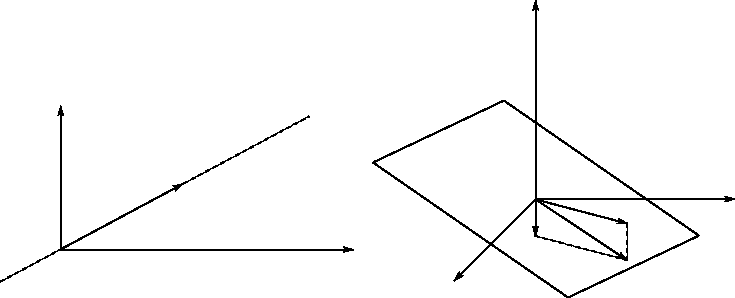
\includegraphics{Images/Sistemi omogenei.pdf}
	\caption{Interpretazione grafica sistemi omogenei}
\end{figure}

\begin{teorema}
	Sia $Ax = b$ un sistema risolvibile. Sia y una soluzione del sistema $ y \in  Sol \left( Ax=b \right) $ detta soluzione particolare. Allora \[
		Sol\left( Ax =b \right)  = \left\{ x = y + x_0 | x_0 \in  Sol\left( Ax=0 \right)  \right\}
	\]
\end{teorema}

\textbf{Dimostrazione:}
Devo dimostrare la seguente doppia implicazione, tenendo presente che $ Ay=b $:
\[
	Ax =0 \Leftrightarrow A \left( x + y \right) = b
\]
\begin{itemize}
	\item $ Ax =0 \Rightarrow A\left( x+y \right) =b $
	      \[
		      A\left( x+y \right) = Ax+Ay =  0+b = b
	      \]
	      Quindi $x+y$ è soluzione del sistema omogeneo $Ax=b$
	\item $ Ax =0 \Leftarrow A\left( x+y \right) =b $
	      \[
		      A\left( x+y \right) = Ax + Ay = b \rightarrow Ax = 0
	      \]
	      Ossia $ x $ deve essere soluzione del sistema omogeneo
\end{itemize}

\section{Matrici delle operazioni elementari}
Per eseguire sulle righe di $A$ un'operazione elementare basta moltiplicare $A$ \underline{a sinistra} per una matrice $A$(detta matrice elementare) ottenuta dalla matrice identica di ordine n $I_n$ applicando su quest'ultima le stesse operazioni che voglio applicare su $A$
\begin{itemize}
	\item \underline{Primo tipo}$S_{ij}A = S_{ij} \rightarrow
		      \begin{bmatrix}
			      1 & 0 & 0 & 0 \\
			      0 & 0 & 1 & 0 \\
			      0 & 1 & 0 & 0 \\
			      0 & 0 & 0 & 1 \\
		      \end{bmatrix} $
	\item \underline{Secondo tipo} $D_j\left( i \right) A \rightarrow S_{ij}=
		      \begin{bmatrix}
			      1 & 0 & 0 \\
			      0 & c & 0 \\
			      0 & 0 & 1
		      \end{bmatrix} $
	\item \underline{Terzo tipo} $E_{ij}\left( c \right) A \rightarrow E_{ij}\left( c \right) =
		      \begin{bmatrix}
			      1 & 0 & 0 \\
			      0 & 1 & c \\
			      0 & 0 & 1
		      \end{bmatrix} $
\end{itemize}
OSS:
\begin{itemize}
	\item $S_{ij}^{-1}= S_{ij}$
	\item $D_j\left( c \right) ^{-1}= D_j\left( \frac{1}{c} \right) $
	\item  $E_{ij}\left( c \right) ^{-1}=R_{ij}\left( -c \right) $
\end{itemize}
\begin{tcolorbox}
	Posso vedere processo di riduzione gaussiana come serie di prodotti matriciali:
	\[
		E_k\left( \ldots \left( E_2 \left( E_1A \right)  \right)  \right) = E_k \ldots E_2 E_1 A = PA
	\]

\end{tcolorbox}

Sia $m=n$. Sia S = rref(A) ossia la sua matrice ridotta. Se $rg\left( A \right) = n \Rightarrow A $ è invertibile
\begin{itemize}
	\item $PA=S=rref\left( a \right) $
	\item Deve essere matrice identica in quanto \textit{pivot} sono $=1$ e $rg\left( A \right) =n$ per questa ragione:
	      \[
		      PA=S=rref\left( a \right) =I_n
	      \]
	\item Siccome $PA=I_n$ posso moltiplicare per $P^{-1}$ da entrambe le parti
	      \[
		      P^{-1}PA=P^{-1}
	      \]
	      \[
		      A=P^{-1} \rightarrow A^{-1}=P
	      \]
\end{itemize}
\subsubsection*{Inverse e metodo per trovare matrice $P$ in un colpo solo}
Supponiamo di volere trovare la matrice $P$ in un solo colpo. Posso agire nel seguente modo:
\begin{itemize}
	\item Creo matrice composta affiancando a destra di $A$ la matrice identica:
	      \[
		      \left( A|I_m \right)
	      \]
	\item Applico riduzione su intera matrice $ \left( A|I_m \right) $
	\item A fianco della matrice $A$ ottengo matrice $P$ in quanto:
	      \[
		      P\left( A|I_m \right) = \left( PA |PI_m \right) = \left( S| P \right) = \left( I_m | P\right)
	      \]
\end{itemize}
\textbf{Esempio}:
\[
	A= \begin{bmatrix}
		1 & 1 & 2  \\
		0 & 1 & -1 \\
		2 & 3 & 1
	\end{bmatrix}
\]
\begin{itemize}
	\item Affianco matrice identica:
	      \[
		      \begin{bmatrix}
			      1 & 1 & 2  & 1 & 0 & 0 \\
			      0 & 1 & -1 & 0 & 1 & 0 \\
			      2 & 3 & 1  & 0 & 0 & 1
		      \end{bmatrix}
	      \]
	\item Riduco intera matrice a scala con metodo di Gauss Jordan:
	      \[
		      \begin{bmatrix}
			      1 & 1 & 2  & 1  & 0  & 0 \\
			      0 & 1 & 1  & 0  & 1  & 0 \\
			      0 & 0 & -2 & -1 & -1 & 1
		      \end{bmatrix}
		      \rightarrow
		      \begin{bmatrix}
			      1 & 0 & 0 & -2 & - \frac{5}{2} & \frac{3}{2}  \\
			      0 & 1 & 0 & 1  & \frac{3}{2}   & -\frac{1}{2} \\
			      0 & 0 & 1 & 1  & \frac{1}{2}   & -\frac{1}{2}
		      \end{bmatrix}
	      \]
\end{itemize}

\begin{teorema}{Invertibilità matrici quadrate }
	Sia $A$ una matrice quadrata $m \times m$ invertibile.

	\underline{Parte 1}: Ogni sistema $Ax = b$ ha un'unica soluzione $x = A^{-1}b$.
	\vskip3mm
	\underline{Parte 2}:
	\[
		A \quad  n\times n  \quad A \text{ è invertibile }  \Leftrightarrow rg\left( A \right) =n
	\]
\end{teorema}

Dimostrazione
\begin{itemize}
	\item \underline{Parte 1}: il sistema $Ax= b$ ha un'unica soluzione uguale a $A^{-1}b$:
	      \begin{itemize}
		      \item Se $x$ è soluzione di $Ax=b$ allora posso ricavare la seguente uguaglianza $\Leftrightarrow$ $A$ è invertibile:
		            \[
			            x =  A^{-1}Ax
		            \]
		      \item Visto che per ipotesi $x$ è soluzione del sistema, $Ax=b$. Ricavo dunque che
		            \[
			            x=A^{-1}b
		            \]
		            quindi il sistema  $Ax=b$ ammette \underline{una sola soluzione} (in quanto $A^{-1}$ è unica) uguale a $A^{-1}b$
	      \end{itemize}
	\item \underline{Parte 2}:
	      \begin{itemize}
		      \item $rg\left( a \right) = n \Rightarrow A$  è invertibile:
		            \begin{itemize}
			            \item Riducendo la matrice $\left( A|I_m \right) $ ottengo $\left( I_m|P \right) $
			            \item Visto che $PA = rref\left( A \right) = I_m$ posso affermare che:
			                  \[
				                  P=A^{-1}
			                  \]
		            \end{itemize}
		      \item $A$ invertibile $ \Rightarrow rg\left( a \right) =n$
		            \begin{itemize}
			            \item Come dimostrato in parte 1, se $A$ è invertibile, allora $Ax=b$ ammette un'unica soluzione
			            \item Se $Ax=b$ ammette un'unica soluzione, necessariamente
			                  \[
				                  rg\left( A \right) =n
			                  \]
		            \end{itemize}
	      \end{itemize}
\end{itemize}
\textbf{Esempio:}
stabiliamo se la seguente matrice è invertibile. Per quali k lo è?
\[
	\begin{bmatrix}
		2 & k & 1  \\
		1 & 0 & 2  \\
		1 & k & -k
	\end{bmatrix}
\]
\begin{itemize}
	\item Affianco matrice $I_n$
	      \[
		      \begin{bmatrix}
			      2 & k & 1  & 1 & 0 & 1 \\
			      1 & 0 & 2  & 0 & 1 & 0 \\
			      1 & k & -k & 0 & 0 & 1 \\
		      \end{bmatrix}
	      \]
	\item Riduco matrice con Gauss-Jordan
	      \[
		      \begin{bmatrix}
			      1 & 0 & 2   & 0  & 1  & 0 \\
			      0 & k & -3  & 1  & -2 & 0 \\
			      0 & 0 & 1-k & -1 & 1  & 1
		      \end{bmatrix}
	      \]
	      \begin{itemize}
		      \item Se $k=0$ ho $rg\left( A \right) =2$ quindi $A$ \underline{non è invertibile}
		      \item Se $k=1$ ho $rg\left( A \right) 2$ qindi $A$ = \underline{non è invertibile}
		      \item Se $k \neq 0,1$ $rg\left( A \right) =3$ quindi $A$ \underline{è invertibile}
	      \end{itemize}
	\item In quest'ultimo caso, con $k \neq 0,1$ posso srivere la matrice in forma ridotta
\end{itemize}
\section{Spazi vettoriali}

\begin{definizione}{Spazio vettoriale}
	Uno \underline{spazio vettoriale} sul campo $\mathbb{K} $ è in insieme $V$, i cui elementi sono detti \underline{vettori}, su cui sono definite una \underline{somma} e una \underline{moltiplicazione per scalare} tali che:
	\begin{itemize}
		\item (V, +) è un gruppo commutativo
		      \begin{itemize}
			      \item associatività
			      \item esistenza elemento nullo
			      \item esistenza inverso
			      \item commutatività
		      \end{itemize}
		\item $\left( V, \times \right) $ deve soddisfare le seguenti proprietà $ \forall k_1,k_2,k_3 \in  \mathbb{K} \quad \forall v_1,v_2,v_3 \in V$:
		      \begin{itemize}
			      \item $\left( k_1+ k_2 \right) v= k_1v+ k_2v $
			      \item $k\left( v_1+v_2 \right) =kv_1+kv_2 $
			      \item $ \left( k_1k_2 \right) k_3= k_1\left( k_2k_3 \right) $
			      \item $1v=v $
		      \end{itemize}
	\end{itemize}
\end{definizione}

\textbf{Esempi:}
\begin{itemize}
	\item $V^2, V^3 \quad \text{ spazi vettoriali in  }\R $
	\item $\R^{n}$ (spazio n-uple ordinate) spazio vettoriale reale
	\item $\C^{n}$ (spazio n-uple ordinate) spazio vettoriale complesso
	\item $M_{mn}\left( \R \right) $
	\item $\R \left[ x \right] = \left\{ f : \R \to \R | f\left( x \right) = a_0 + a_1x + a_2 x\ldots + a_dx^{d}, a_0, a_1 \ldots a_d \in  \R\right\} $ \underline{polinomi}
	      \begin{itemize}
		      \item $\left( f+q \right) \left( x \right)= f\left( x \right) + q\left( x \right) = \left( a_0 + b_0 \right) + \left( a_1+b_1 \right) x + \ldots \left( a_d + b_d \right) x^{d} $
		      \item $\left( kf \right) \left( x \right) = kf\left( x \right) $
	      \end{itemize}
	\item $\C\left( \R \right) = \left\{ f:\R \to \R  | f \text{ continua } \right\} $ (insieme funzioni continue)
\end{itemize}
\subsection{Sottospazi vettoriali}
\begin{definizione}{Sottospazio vettoriale}
	Sia $V$ una spazio vettoriale (in $\mathbb{K}$). Sia $W \subseteq V$ un sottoinsieme non vuoto. $W$ è detto \underline{sottospazio vettoriale} di $V$ se
	\begin{itemize}
		\item $\forall w_1, w_2 \in W \quad w_1+w_2 \in  W$
		\item $\forall w \in  W, \forall k \in  \mathbb{K}, \quad kw \in  W$
	\end{itemize}
\end{definizione}
OSS: $W$ è spazio vettoriale, rispetto alle operazioni di $V$: ogni \underline{sottospazio} vettoriale è anche uno \underline{spazio} vettoriale\\
OSS: Ogni sottospazio contiene $0$ (vettore nullo di $V$):
\[
	\text{ se } w \in  W , 0w=0 \in W
\]
\textbf{Esempi:}
\begin{itemize}
	\item $Sol\left( Ax= 0\right) \subseteq R^{n}$ è sottospazio: immaginati piano per origine in  $\R^{3}$. Il prodotto per scalare soddisfa le proprietà necessarie ed è presente l'elemento nullo in quano il piano \underline{passa per l'origine}.
	\item $Sol\left( Ax=b \right) \quad \text{ con } b \neq 0$ non è sottospazio vettoriale: immaginando il piano in $\R^{3}$ posso affermare che
	      \begin{itemize}
		      \item Non è presente l'elemento nullo
		      \item $kv \not\in Sol\left( Ax=b \right) $ se $v \in Sol\left( Ax=b \right) $
	      \end{itemize}
	\item Insieme delle \underline{matrici simmetriche} $A=A^{T}$ reali di ordine $n$ è un sottopspazio di $M_n\left( \R \right) $
	\item  \underline{Polinomi} a coefficienti reali di grado $ < n$ sono sottospazio di $\R \left[ x \right] $ (chiamato $ \R_n\left[ x \right] $)
	\item $\R\left[ x \right] $ è sottospazio di $C\left( \R \right) $ (i polinomi sono sottospazio delle funzioni in generale)
\end{itemize}
\subsection{Esempio campo finito}
Consideriamo il campo $ \mathbb{F}=\left\{ 0,1 \right\} $ ossia un campo finito con soli due elementi. Per far si che questo sia un campo devo tenere in mente una sola regola:
\[
	1+1=0
\]
in modo tale che ogni operazione possibile dia risultato $k \in  \mathbb{F}$
\vskip3mm
Consideriamo il sistema lineare in $ \mathbb{F}$ :
\[
	\begin{cases}
		x_1+x_2=1 \\
		x_1-x_2=1
	\end{cases}
	\text{ con matrice dei coefficienti }
	\begin{bmatrix}
		1 & 1  \\
		1 & -1
	\end{bmatrix}
\]
risolvo con Gauss-Jordan e ottengo
\[
	\begin{bmatrix}
		1 & 1 & 1 \\
		0 & 0 & 0
	\end{bmatrix}
\]
Per Rouché-Capelli so che in numero di variabili indipendendi sono uguali a $null\left( A \right) = n-rg\left( A \right) = 1$. Le soluzioni tuttavia vanno ricercate solo all'interno di $ \mathbb{F}$. Il numero di soluzioni \underline{non} è dunque \underline{infinito} come sarebbe in $\R$, bensì $2^{1}=2$
\[
	Sol\left( Ax=b \right) = \left\{ \left( 1,0 \right) , \left( 0,1 \right)  \right\}
\]

\section{Basi, generatori e indipendenza lineare}

\begin{definizione}{Combinazione lineare}
	Un vettore $v \in  V$ è \underline{combinazione lineare} dei vettore $ v_1,\ldots , v_k \in  V$ mediante i coefficienti $c_i \in  \mathbb{K}$ se
	\[
		v = c_1v_2+ \ldots + c_k v_k
	\]
\end{definizione}
Useremo il simbolo $ \left<v_1,\ldots,v_k \right>$ per indicade \underline{ogni possibile combinazione lineare} dei vettori $v_1,\ldots,v_k$
\[
	\left<v_1,\ldots , v_k	\right> = \left\{ c_1,v_1+\ldots+c_kv_k | c_1,\ldots,c_k \in  \mathbb{K}\right\}
\]
\textbf{Esempi}:
\begin{enumerate}
	\item Due vettori di $\R^{3}$ generano il sottospazio vettoriale coicidente ad \underline{un piano}. Ad esempio:
	      \[
		      v_1=\left( 2,3,1 \right) \quad v_2=\left( 0,2,1 \right)
	      \]
	      scrivendo combinazione lineare per $c_1,c_1 \in  \R$ ottengo che questi vettori generano il sottospazio
	      \[
		      W = \left<v_1,v_2 \right> \left\{ 2c_1,3c_1+2c_2,c_1+c_2 | c_1,c_2 \in  \R \right\}
	      \]
	      ossia il piano passante per l'origine (normalmente, per ricavare l'equazione di un piano dovrei traslare la combinazione lineare forzando il passaggio per un punto)
	\item Come dimostro che $\left<x+1,x-1, x^2-1 \right>$ genera $\R_n\left[ x \right] $?
	      \begin{itemize}
		      \item Osservo che la base canonica di $\R_n\left[ x \right] $ è data da $\left( 1,x,x^2 \right) $
		      \item Se riesco a ricavare ogni elemento della base canonica per combinazione lineare sono a posto. Ciò è vero in quanto \underline{la combinazione lineare di elementi ottenuti per combinazione lineare di $x,y,z$ sarà sempre combinazione lienare di $x,y,z$}
	      \end{itemize}
\end{enumerate}

\begin{definizione}{Base dello spazio vettoriale}
	Sia $V$ uno spazio vettoriale in $\mathbb{K}$. Un insieme di vettori  $v_n$ viene detto \underline{base }di $V$ se ogni elemento $v \in  V$ si può scrivere \underline{in modo unico} come combinazione lineare.
	\[
		v = x_1v_1 +\ldots n_nv_n = \sum_{i=1}^{n} x_iv_i
	\]
	Tutte le basi di uno spazio vettoriale $V$ hanno lo \underline{stesso} numero di elementi. Tale numero è detto \underline{dimensione} dello spazio vettoriale
	\vskip3mm
	I coefficienti $x_1 \ldots x_n$ della combinazione lineare si dicono \underline{cooerdinate di $V$ rispetto alla base} $\left\{ v_1\ldots v_n \right\} $
\end{definizione}

\begin{definizione}{Insieme generatore}
	Un insieme di vettore $ v_1,\ldots,v_m$ è detto \underline{insieme generatore} di $V$ se ogni vettore $v$ di $V$ si può scrivere come combinazione lineare:
	\[
		x_1v_1+x_2v_2+\ldots+v_mv_m =  \sum_{i=1}^{n} x_iv_i
	\]
	la differenza rispetto ad una base è che un vettore $v \in  V$ può essere ottenuto tramite diverse coordinate
\end{definizione}

\begin{definizione}{Vettori linearmente indipendenti}
	Un insieme di vettori $v_1,\ldots, v_k$ è detto \underline{linearmente indipendente} se il vettore nullo si piò scrivere come combinazione lineare dei $v_i$ solo scegliendo coefficienti  \underline{tutti nulli}
	\[
		a_1v_1+a_2c_2+\ldots+ a_kv_k=0 \Leftrightarrow a_1\ldots a_k=0
	\]
	se i vettori non sono linearmente indipendenti questi si dicono \textit{linearmente dipendenti}
\end{definizione}

OSS: un gruppo di vettori sono linearmente dipendenti se e solo se almeno uno di questi si può scrivere come combinazione lineare degli altri
\vskip3mm
Esempio: stabilisci se i seguenti vettori sono linearmente indipendenti:
\[
	v_1= \left( 1,1,0 \right) \quad v_2=\left( 0,1,1 \right) \quad v_3=\left( 1,-1,-2 \right)
\]
Basterà trovare le soluzioni dell'equazione $a_1v_2+a_2v_2+a_3v_3=0$, equivalente al sistema $Ma=0$ dove
\[
	M=
	\begin{bmatrix}
		1 & 0 & 1  \\
		1 & 1 & -1 \\
		0 & 1 & -2
	\end{bmatrix}
	\quad
	a =
	\begin{bmatrix}
		a_1 \\
		a_2 \\
		a_3
	\end{bmatrix}
\]
risolvendo tramite Gauss-Jordan mi accorgo che il sistema ha infinite soluzioni che dipendono da $a_3$, ossia la unica variabile libera:
\[
	\begin{bmatrix}
		1 & 0 & 1  \\
		0 & 1 & -2 \\
		0 & 0 & 0
	\end{bmatrix}
\]
l'insieme è quindi dipendente con soluzioni: $\left( -a_3,2a_3,a_3 \right) $

\begin{teorema}{Criterio affinche un generatore sia base}
	Un insieme $\left\{ v_1,\ldots,v_n \right\} $ di elementi di $V$ è una base di $V \Leftrightarrow $ s è un generatore di $V$ \underline{linearmente indipendente}
\end{teorema}
OSS:
\begin{itemize}
	\item Nel piano due vettori sono LI se e solo se non appartengono alla stessa retta.
	\item Nello spazio tre vettori sono LI se e solo se non appartengono allo stesso piano:
	\item Le basi canoniche di una matrice o di una n-upla sono linearmente indipendenti:
	      \[
		      \left[\begin{array}{lll}1 & 0 & 0 \\ 0 & 0 & 0\end{array}\right],\left[\begin{array}{lll}0 & 0 & 0 \\ 1 & 0 & 0\end{array}\right],\left[\begin{array}{lll}0 & 1 & 0 \\ 0 & 0 & 0\end{array}\right],\left[\begin{array}{lll}0 & 0 & 0 \\ 0 & 1 & 0\end{array}\right],\left[\begin{array}{lll}0 & 0 & 1 \\ 0 & 0 & 0\end{array}\right],\left[\begin{array}{lll}0 & 0 & 0 \\ 0 & 0 & 1\end{array}\right]
	      \]

\end{itemize}
\begin{definizione}{Gruppo finitamente generato}
	Se $V$ è finitamente generato (esiste un numero finito di generatori ) $ \Rightarrow V$ ha una base
\end{definizione}
Esempio: $V = \R\left[ x \right] \rightarrow $ \underline{non è finitamente generato}
in quanto:
\[
	\left\{ p_1,\ldots,p_m \right\} = \sum_{k=0}^{m} a_ip_i
\]
tramite questi generatori posso ottenere polinomi di grado massimmo $= m$
\vskip3mm
OSS:
\[
	V\left\{ 0 \right\}  \text{ è finitamente generato ma non ha basi }
\]
\subsection{Rango e dimensione}
Vi è una relazione ben specifica fra \underline{rango} di una matrice e  \underline{dimensione} dello spazio vettoriale definito dalle sue righe non nulle.
\begin{itemize}
	\item Sia $A$ una matrice di rango $r$, ossia una matrice con $r$ pivot
	\item Sia $S= rref\left( A \right) $ la sua matrice a scalini. Questa matrice avrà $r$ righe non nulle
	\item Le righe $S_1,\ldots, S_r$ sono \underline{linearmente indipendenti} in quanto per annullare la colonna contenente il pivot k-esimo devo moltiplicare per $0$ la k-esima riga
	\item Essendo $S_1,\ldots,S_r$ linearmente indipendenti posso affermare che:
	      \[
		      r=rg\left( A \right) = dim \left<S_1,\ldots,S_r \right>
	      \]
	\item Visto che la matriche $ S$ è ottenuta tramite operazioni elementari, ossia eseguendo combinazioni lineari fra le sue righe, posso affermare che
	      \[
		      \left<A_1,\ldots,A_r \right> = \left<S_1,\ldots,S_r \right>
	      \]
\end{itemize}
NB: di fatto la riduzione a scalini della matrice $ A $ consiste nell' eseguire operazioni di combinazione lineare fra le sue righe fino ad ottenere i vettori della sua base canonica. Risulta quindi evidente che il rango equivale alla dimensione dello spazio delle righe di $ A $

\begin{teorema}{Rango matrice trasposta}
	Lo spazio delle righe e lo spazio delle colonne di $A$ hanno la stessa dimensione, ossia:
	\[
		rg\left( A \right)  = rg\left( A^{T} \right)
	\]
\end{teorema}

Implicazioni:
\begin{itemize}
	\item Immagino di avere k vettori $v_1,\ldots,v_k$ e di voler verificare quali di questi sono \textit{linearmente indipendenti}: ho \underline{2 metodi}:
	      \begin{enumerate}
		      \item Creo la matrice che ha come \underline{righe} i vettori $v_1,\ldots,v_k$ e calcolando la sua matrice ridotta ottengo $k$ righe non nulle che individuano \underline{una base}
		      \item Creo una matriche che ha come \underline{colonne} i vettori $v_1,\ldots,v_k$ e calcolando la sua \textit{matrice ridotta} ottengo più informazioni:
		            \begin{itemize}
			            \item Le colonne contenenti i \textit{pivot} costituiscono le basi canoniche dell'insieme individuato dai vettori di partenza
			            \item Le colonne \underline{non} contennti i \textit{pivot} individuano i \underline{le coordinate} per ottenere la j-esima colonna secondo la base trovata
		            \end{itemize}
	      \end{enumerate}
\end{itemize}
Esempio: in $\mathbb{R}^4$, siano
$$
	v_1=(2,-1,0,1), v_2=(1,1,0,1), v_3=(1,-2,0,0), v_4=(-1,2,2,1), v_5=(0,3,2,2)
$$
La matrice $4 \times 5$ con colonne $v_1, v_2, v_3, v_4, v_5$ ha forma ridotta
$$
	S=\left[\begin{array}{rrrrr}
			1 & 0 & 1  & 0 & 0 \\
			0 & 1 & -1 & 0 & 1 \\
			0 & 0 & 0  & 1 & 1 \\
			0 & 0 & 0  & 0 & 0
		\end{array}\right]
$$
\begin{itemize}
	\item Le colonne $1,2,4$ contengono le basi canoniche. Interpreta il sistema come "la somma di ogni componente di ogni vettore $=0$ ". Se il sistema fosse composto solo dai vettori $1,2,4$, questo avrebbe una sola soluzione. I vettori $1,2,4$ sono quindi \underline{LI} per definizione
	\item Le colonne $3,5$ contengono invece le coordinate secondo la base $\left\{ v_1,v_2,v_4 \right\} $ per ottenere rispettivamente $v_3$ e $v_5$
\end{itemize}

Dato un spazio vettoriale $V$ con una base $B=\left\{ v_1,\ldots,v_n \right\} $. Per definizione di base ogni vettore in $V$ si scrive come \underline{combinazione lineare} fra i vettori della base:
\[
	v= \sum_{k=1}^{n} x_iv_i
\]
Si può scrivere che
\[
	v = \left( x_1,\ldots,x_n \right) _B
\]
ossia che il vettore v è dato dalla combinazione lineare fra la base v e  le \underline{coordinate} $x_1,\ldots,x_n$
\vskip3mm
La n-upla contentente le coordinate di $v$ rispetto alla base $B$ si può scrivere come:
\[
	T_B\left( v \right)
\]
\hr
Esempio:
Dimostriamo che la seguente è una base di $\R^{3}$
\[
	\left\{ v_1 = \left( 2,-1,0 \right) , v_2 = \left( -1,2,1 \right) , v_3=\left( 0,0,1 \right)  \right\} = B
\]
\begin{itemize}
	\item Sia LI :
	      \[
		      M = \left[ v_1,v_2,v_3 \right] =
		      \begin{bmatrix}
			      2  & -1 & 0 \\
			      -1 & 2  & 0 \\
			      0  & 1  & 1
		      \end{bmatrix}
	      \]
\end{itemize}
\subsection{Proprietà basi di $\R^{n}$}
\label{sub::proprietàbasi}
\begin{enumerate}
	\item $m$ vettori di $\R^{n}$ sono necessariamente \underline{linearmente dipendenti} se $m > n$
	\item n vettori \underline{linearmente indipendenti }in $\R^{n}$ sono necessariamente una base di $\R^{n}$
	\item Siano $v_1,\ldots, v_m$ vettori \underline{linearmente indipendenti} di $\R^{n}$ con $m<n$. Allora l'insieme $\left\{ v_1,\ldots,v_m \right\} $ può essere \underline{completato} aggiungendo $n-m$ vettori di $ \R^{n}$
\end{enumerate}
Dimostrazioni:
\begin{enumerate}
	\item Creo matrice $M = \begin{bmatrix}
			      v_1 & \ldots & v_m \\
		      \end{bmatrix}
	      $
	      con  $m > n$
	      \begin{itemize}
		      \item Questa matrice ha rango = $min\left( n,m \right) =n$
		      \item Per forza di cose avrò almeno una variabile libera, ad il sistema omogeneo associato avrà infinite soluzioni.
		            \[
			            \left\{ v_1,\ldots,v_m \right\} \text{ non possono essere LI }
		            \]
	      \end{itemize}
	\item Dati n vettori $v_1,\ldots,v_n$ e un vettore $ \in  \R^{n}$ v creo sistema associato
	      \[
		      M=\begin{bmatrix}
			      v_1 & \ldots & v_k
		      \end{bmatrix}
		      =v
	      \]
	      \begin{itemize}
		      \item $M$ ha rango $=n$ in quanto i vettori $v_1,\ldots,v_k$ sono \underline{LI}
		      \item Per questa ragione il sistema $Mx=v$ ha un'unica soluzione, ossia \underline{ $v_1,\ldots,v_k$ sono una base}
	      \end{itemize}
	\item Considero la matrice $M= \begin{bmatrix}
			      v_1 & \ldots & v_k & e_1 & \ldots & e_n \\
		      \end{bmatrix}
	      $
	      \begin{itemize}
		      \item Questa matrice ha rango $=n$ in quanto le ultime $n$ colonne sono \underline{LI}
		      \item Le prime $m$ colonne sono uguali a $e_1,\ldots,e_m$ in quanto $v_1,\ldots,v_m$ sono  \underline{LI}
		      \item  Visto che il rango è $n$, ottengo per forza altri $n-m$ \textit{pivot}, in corrispondenza delle colonne che devo aggiungere per completare la base
	      \end{itemize}
\end{enumerate}
Esempio:per completare l'insieme indipendente
$$
	\left\{v_1=(1,0,2,1), v_2=(1,1,-2,-1)\right\}
$$
a una base di $\mathbb{R}^4$, basta considerare la riduzione per righe
$$
	\operatorname{rref}\left[\begin{array}{rrrrrr}
			1 & 1  & 1 & 0 & 0 & 0 \\
			0 & 1  & 0 & 1 & 0 & 0 \\
			2 & -2 & 0 & 0 & 1 & 0 \\
			1 & -1 & 0 & 0 & 0 & 1
		\end{array}\right]=\left[\begin{array}{rrrrrr}
			1 & 0 & 0 & 1  & 0 & 1  \\
			0 & 1 & 0 & 1  & 0 & 0  \\
			0 & 0 & 1 & -2 & 0 & -1 \\
			0 & 0 & 0 & 0  & 1 & -2
		\end{array}\right]
$$
Le colonne 1,2,3,5 sono indipendenti. Quindi I'insieme
$$
	\left\{v_1, v_2, e_1, e_3\right\}
$$
forma una base di $\R^{4}$. Non è necessario ottenere una matrice ridotta per individuare le colonne indipendenti, è sufficiente una matrice a scalini

\begin{teorema}{Teorema della base di $\R^n$}
	Ogni base di $\R^{n}$ contiene \underline{esattamente} n elementi
\end{teorema}

Dimostrazione
\begin{itemize}
	\item  $m$ vettori di $\R ^{n}$ se $m > n$ sono necessariemente \underline{linearmente dipendenti} allora \underline{una base non può conenere più di $n$ elementi} (sezione \ref{sub::proprietàbasi}, proposizione 1)
	\item Un insieme di $m$ vettori con $m<n$ può essere completato con $n-m$ vettori (sezione \ref{sub::proprietàbasi}, proposizione 3)
	\item Siccome i vettori che aggiungo sono linearmente indipendendi, questi non possono essere creati con combinazione lineare dai primi $m$. Per questo i primi  $m$ vettori non possono essere generatori dello spazio $\R^{n}$
\end{itemize}
\section{Somma e intersezione sottospazi}
\subsection{Intersezione}
L'intersezione di due sottospazi è sempre sottospazio
\begin{itemize}
	\item Prendo 2 vettori $ v_1,v_2 \in V_1 \cap V_2$ ossia appartenenti all'intersezione degli spazi
	\item Visto che $ v_1,v_2 \in  V_1 $ allora ogni loro combinazione lineare sta in $ V_1 $
	\item Visto che $ v_1,v_2 \in  V_2 $ allora ogni loro combinazione lineare sta in $ V_2 $
	\item Visto che ogni combinazione lineare sta sia in $ V_1 $ che in $ V_2 $ allora ogni combinazione lineare sta in $ V_1 \cap V_2 $. \underline{L'intersezione è sottospazio}
\end{itemize}

\subsection{Unione}
L'unione insiemistica di sottospazi non è sottospazio, basti pensare al seguente caso in $\R^{2}$
\begin{center}
	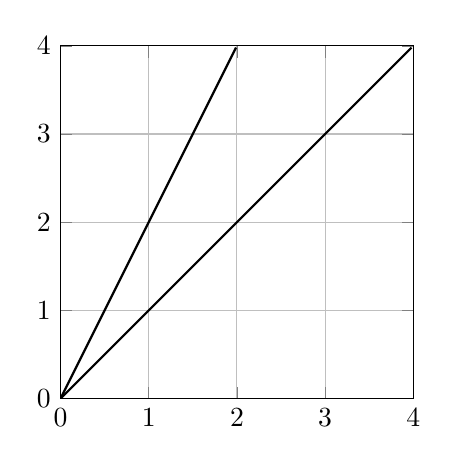
\begin{tikzpicture}
		\begin{axis}[
				xmin=0, xmax=4,
				ymin=0,ymax=4,
				restrict y to domain = 0:4, domain=0:4, width=0.5\textwidth, height=0.5\textwidth, grid=major, samples=200]
			\addplot[black, thick] {x};
			\addplot[black, thick] {2*x};
		\end{axis}
	\end{tikzpicture}
\end{center}
Se prendo due vettori sulle due rette mi rendo conto che la loro somma non ricade all'interno di nessuna delle due rette. Posso però definire una \underline{somma fra sottospazi}
\begin{definizione}{Somma di sottospazi}
	La somma di $V$ e $W$ è l'insieme
	\[
		V + W = \left\{ v \in  V | v = u + w, v \in V, w \in  W \right\}
	\]
	ossia la somma di ogni vettore in $W$ con ogni vettore di $V$
\end{definizione}

\begin{formula}{Formula di Grassmann}
	\[
		dim\left( V \right) + dim\left( W \right)  = dim\left( V \cap W \right) + dim\left( V + W \right)
	\]
\end{formula}
Esempio:
Considero due spazi vettoriali:
\[
	V=\left\{ p \in  \R_3\left[ x \right] | x p '' = 2p'  \right\}
\]
\[
	W = \left\{ p \in  \R_3 \left[ x \right] | p\left( 2 \right) = p\left( 4 \right) = 0 \right\}
\]
\begin{itemize}
	\item Caso 1:
	      \begin{itemize}
		      \item Prendo polinomio generico
		      \item Derivo
		      \item Risolvo sistema
	      \end{itemize}
	\item Caso 2:
	      \begin{itemize}
		      \item Risolvo sistema che impone che il polinomio si annulli in  2 e in 4
		      \item Alternativamente posso scrivere i polinomi nel seguente modo
		            \[
			            \left( x-2 \right) \left( x-4 \right) \quad \text{ e } \quad x\left( x-2 \right) \left( x-4 \right)
		            \]
	      \end{itemize}
\end{itemize}
\subsection{Interpolazione polinomiale}
Dati $ n $ punti $\left( x_1, y_1 \right) , \ldots, \left( x_n, y_n \right) $ voglio trovare $p\left( x \right) \in  \R\left[ x \right] $ tali che
\[
	p\left( x_i \right) = y_i \quad \forall i = 1,\ldots, n
\]
noto che non posso rappresentare $R\left[ x \right] $ con una base che abbia un numero finito di elementi. Restringo quindi il grado del polinomio. Si può dimostrare che la soluzione \underline{è unica} in $\R_{n-1}\left[ x \right] $ (pensa al teorema fondamentale dell'algebra, un polinomio di grado $n$ ha $n$ zeri).
\vskip3mm
La logica è la seguente:
\begin{itemize}
	\item Creo tramite la cosiddetta \textit{base di lagrange} $n$ polinomi $f_1\left( x \right),\ldots, f_{n - 1}\left( x \right) $ che abbiano le seguenti proprietà:
	      \begin{itemize}
		      \item $f_i\left( x_i \right) =1$
		      \item $f_i\left( x_j\right) = 0 \quad \forall j = 1\ldots n-1, j \neq i$
	      \end{itemize}
	\item Noto che il polinomio $f_i\left( x \right) $ vale zero "sotto" ad ogni punto meno che sotto a $x_i$. Se lo sommo con altri polinomi $f_1\left( x \right) ,\ldots, f_{n-1}\left( x \right) $ posso ottenere un polinomio che passa per tutti i punti $x_1,\ldots, x_{n}$
	      i
\end{itemize}
Introduciamo la base di Lagrange:
\begin{definizione}{Base di langrange}
	La base di lagrange mi permette di trovare un polinomio $f_i\left( x \right) $ che valga \underline{1} sotto a $x_i$, mentre \underline{0} sotto ogni altra $x_1,\ldots,x_n$
	\[
		B = \left\{ f_1,\ldots,f_n \right\}
	\]
	\[
		f_i\left( x \right) = \prod_{j=1}^{n} \frac{x-x_j}{x_i - x_j} \quad  \text{ con } j \neq i
	\]
\end{definizione}
Nota che la base di lagrange $f_i\left( x \right) $ è un \underline{polinomio} che vale 0 in $x_j$ per $j=1,\ldots,n$ mentre vale 1 in $x_i$. Chiaramente quindi le basi di lagrange sono linearmente indipendenti e ci permettono di creare un polinomio che passi per tutti i punti indicati.
\vskip3mm
Esempio: dati tre punti $\left( 2,1 \right)  \left( 4,2 \right)  \left( 5,0 \right) $ si trovi un polinomio che passi per essi.
\begin{itemize}
	\item Cerco base di Lagrange:
	      \begin{align*}
		      f_1 \left( x \right) & = \frac{x-x_2}{x_1-x_2} \frac{x-x_3}{x_1-x_3} =\frac{1}{6}\left( x-4 \right) \left( x-5 \right)  \\
		      f_2 \left( x \right) & = \frac{x-x_1}{x_2-x_1} \frac{x-x_3}{x_2-x_3} = \frac{1}{2}\left( x-2 \right) \left( x-5 \right) \\
		      f_3\left( x \right)  & = \frac{x-x_1}{x_3-x_1} \frac{x-x_2}{x_3-x_2}=\frac{1}{3}\left( x-2 \right) \left( x-4 \right)
	      \end{align*}
	\item Una volta trovata la base di lagrange posso fare combinazione lineare con $f_1, f_2, f_3$. Il polinomio finale è:
	      \[
		      y_1f_1\left( x \right)  + y_2f_2\left( x \right) + y_3f_3\left( x \right) = 1f_1\left( x \right) + 2f_2\left( x \right) + 0 f_3\left( x \right)
	      \]
	\item Eseguendo i conti ottengo:
	      \[
		      p\left( x \right) = \left( x-5 \right) \left( -\frac{5}{6}x + \frac{4}{3} \right)
	      \]
	\item Volendo posso verificare che
	      \begin{align*}
		      f\left( x_1 \right) & =  f\left( 2 \right) =1 \\
		      f\left( x_2 \right) & =  f\left( 4 \right) =2 \\
		      f\left( x_3 \right) & = f\left( 5 \right) =0
	      \end{align*}
\end{itemize}
\section{Determinante}
Premessa:
\begin{itemize}
	\item Il determinante è definito solo per matrici quadrate
	\item L'interesse del determinante è più teorico che pratico
\end{itemize}
Esempio:
Sia $A \quad 2 \times 2
	\begin{bmatrix}
		a & b \\
		c & d
	\end{bmatrix}
$
Ha righe \underline{linearmente indipendenti} (ossia $rg\left( A \right) =2$) se e solo se:
\[
	D=ad-bc \neq 0
\]
Se il determinante $D$ è diverso da 0 posso definire la quantità $\frac{1}{D}$. Noto che la matrice
\[
	B=\frac{1}{D}\begin{bmatrix} d & -b \\ -c & a \end{bmatrix}
\]
è la matrice inversa di $A$ e posso verificarlo moltiplicandola per $A$
\hr
Perchè se $ \det\left( A \right) = 0 $ allora le colonne sono \underline{linearmente dipendenti?}
\begin{itemize}
	\item $ \det\left( A \right) = ad-bc = 0  \rightarrow ad= bc$
	\item 	Se $ c, d \neq 0 $ il vale la seguente relazione:
	      \[
		      \frac{a}{c}=\frac{b}{d} = t \quad \rightarrow \quad \left( a,c \right) = t\left( c,d \right)
	      \]
\end{itemize}
I vettori $ \left( a,c \right)  $ e $ \left( c,d \right)  $ sono proporzionali se $ \det\left( A \right) =  0  $

\begin{definizione}{Determinante}
	Sia $A \quad n \times n$. Il  \underline{determinante} di $A$  viene definito in maniera ricorsiva nel seguente modo:
	\begin{itemize}
		\item Se $n=1$, $\det\left[ a_{11} \right]  =a_{11}$
		\item Se $n >1$ $\det\left( A \right) = \sum_{i=1}^{n} a_{i_1}a_{i_1}'$ dove $a_{i_1}'= \left( -1 \right) ^{i+1} \det \left( A_{i_1} \right) $. La matrice $A_{i_1}$ è ottenuta da $A$ toglienda la \textit{i-esima} riga e la \underline{prima} colonna
	\end{itemize}
\end{definizione}
NB: il calcolo del determinante ha complessità \underline{fattoriale}, quindi è possibile farlo solo su matrici molto piccole
\vskip3mm
\textbf{Esempio 1:}
Data la matrice:
\[
	\det
	\begin{bmatrix}
		2  & 1 & 0 \\
		-1 & 0 & 3 \\
		1  & 1 & 1
	\end{bmatrix}
	=2 \det\begin{bmatrix} 0&3 \\1 & 1  \end{bmatrix} -1\left( -1 \right) \det\begin{bmatrix} 1&0\\1 &1 \end{bmatrix} +1\det\begin{bmatrix} 1&0\\0&3 \end{bmatrix}
\]
\textbf{Esempio 2:}
Provando a ridurre una matrice triangolare alta (ossia ua matrice che abbia zeri nella parte inferiore alla diagonale principale non compresa), ottengo che
\[
	\det(A) = \prod_{i=1}^{n}  a_{ii}
\]
osserviamo che
\[
	\det\left( A \right) = \det
	\begin{bmatrix}
		3 & 2  & 1 & 0  \\
		0 & -1 & 3 & 1  \\
		0 & 0  & 1 & -1 \\
		0 & 0  & 0 & 4  \\
	\end{bmatrix}
	= 3 \det
	\begin{bmatrix}
		-1 & 3 & 1  \\
		0  & 1 & -1 \\
		0  & 0 & 4
	\end{bmatrix}
	=3 \cdot -1 \cdot \det
	\begin{bmatrix}
		1 & -1 \\
		0 & 4
	\end{bmatrix}
	= 3 \left( -1 \right) 1\left( 4 \right)
\]
in quanto l'unico elemento che può essere non nullo è l'elemento sulla diagonale.
\subsection{Proprietà determinante}
\label{proprietàDet}

\begin{itemize}
	\item $ \det \left( A \right) = - \det \left( B \right)  $ dove $ B $ è una matrice ottenuta scambiando due righe di $ A $
	\item $ \det \left( B \right) = c \det \left( A \right)  $ se $ B $ è ottenuta moltiplicando una riga di $ A $ per lo scalare $ c $
	\item $ \det \left( B \right)  = \det\left( A \right) $ se $ B $ è ottenuta aggiungendo due righe di $ A $, moltiplicando la seconda per una scalare $ c $
	      \hr
\end{itemize}
\subsubsection*{Dimostrazione 1}
La dimostrazione di basa sulla seguente idea, da applicare ricorsivamente: prendo una matrice $ A $ e scambio due delle sue righe (chiamo quest'ultima matrice $ B $).
\[
	A=
	\begin{bmatrix}
		a & \ldots \\b& \ldots\\c& \ldots  \\d& \ldots\\e& \ldots\\f & \ldots
	\end{bmatrix}
	\quad
	B= S_{2 , 5}A=
	\begin{bmatrix}
		a & \ldots \\e& \ldots\\c& \ldots  \\d& \ldots\\b& \ldots\\f & \ldots
	\end{bmatrix}
\]
Poi faccio i seguenti ragionamenti, che dimostrano \underline{per induzione} questa proprietà:
\begin{itemize}
	\item Se voglio che il rango di $ B $ sia l'opposto di quello di $ A $ nello sviluppo devo avere che ogni $ a_{i 1} \det A_{i 1} $ sia l'inverso del corrispettivo elemento calcolato in $ B $
	\item Ho più casi:
	      \begin{itemize}
		      \item Se la riga $ i $ non è una delle due scambiate il suo \underline{complemento algebrico} sarà una matrice anch'essa con due righe invertite. Il segno dato da $ \left( -1 \right) ^{i+1} $ non è alterato in quanto scambiando due righe non altero gli indici ai quali sono posizionati gli elementi non alterati.
		            \vskip3mm
		            In questo caso gli elementi  $a,c,d,f$ nel calcolo del determinante di $ B $ danno un risultato opposto di quello di $ A $
		      \item Prendendo in considerazione gli elementi che vengono scambiati devo tenere conto di una cosa carina:
		            \begin{itemize}
			            \item Considera ciò lo sviluppo secondo $ b $ nella matrice $ A $ e nella matrice $ B $. Questo sarà uguale a $ b \cdot \left( -1 \right) ^{i+1} $. Quindi se la differenza fra gli indici di $ a $ e $ b $ è un numero dispari il segno sarà invertito:
			                  \[
				                  \det \left( A \right)  = \ldots + b \cdot\left( -1 \right)+\ldots \quad \det \left( B \right)  = \ldots + b \cdot \left( 1 \right) +\ldots
			                  \]
			            \item Il complemento algebrico di $b$ $ B $ sarà uguale a quello di $ b $ in $ A $, ma andranno fatte \underline{$ n $ operazioni di scambio riga}. $ n $ è dispari se la differenza degli indici delle righe scambiate è dispari. In caso contrario è pari. La seguente immagine può spiegare meglio:
			                  \begin{center}
				                  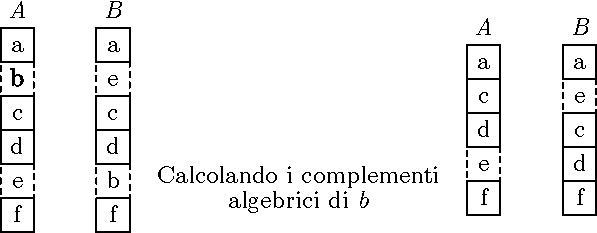
\includegraphics{Images/DimDeterminante1.pdf}
			                  \end{center}
			                  \begin{center}
				                  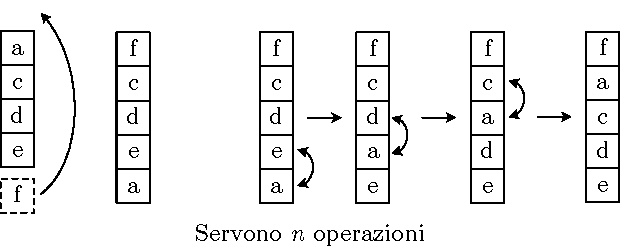
\includegraphics{Images/DimDeterminante1.1.pdf}
			                  \end{center}
			            \item Quindi se $ n $ è pari, assumendo che la proprietà che stiamo cercando di dimostrare sia vera, avverranno $ n $ scambi, e il segno non cambiera. Contrariamente, il segno sarà opposto.
		            \end{itemize}
		      \item Riassumento, sia $ n $ la differenza fra gli indici di $ a $ e di $ b $ -1(ossia il numero di "blocchetti" che saparano $ a $ e $ b $ , allora
		            \vskip3mm
		            \begin{forest}
			            [n, for tree={forked edges, draw=gray!20, align=left, grow'=0}
					            [pari
							            [Coefficiente moltiplicativo \underline{diverso}]
							            [Determinante del complemento \underline{non} si inverte]
					            ]
					            [dispari
							            [Coefficiente moltiplicativo \underline{uguale}]
							            [Determinante del complemento si inverte]
					            ]
			            ]
		            \end{forest}
	      \end{itemize}
\end{itemize}
\subsubsection*{Dimostrazione 2}
Procedo per induzione come nella dimostrazioni precedente:
\[
	A=
	\begin{bmatrix}
		a & \ldots \\b& \ldots\\c& \ldots  \\d& \ldots\\e& \ldots\\f & \ldots
	\end{bmatrix}
	\quad
	B= D_2\left( k \right) =
	\begin{bmatrix}
		a & \ldots \\k\cdot b& \ldots\\c& \ldots  \\d& \ldots\\e& \ldots\\f & \ldots
	\end{bmatrix}
\]
\begin{itemize}
	\item Se nello sviluppo la riga presa in considerazione non è quella moltiplicata per lo scalare, ottengo che la costante moltiplicativa rimane la stessa, mentre il \underline{complemento algebrico} è una matrice con una riga moltiplicata per $ k $
	\item Se nello sviluppo la riga presa in considerazione non è quella moltiplicata per lo scalare ottengo che la costante moltiplicativa è moltiplicata a sua volta per $ k $, mentre il complemento algebrico rimane invariato
\end{itemize}
Raccogliento $ k $ ottengo la proprietà enunciata
\subsubsection*{Dimostrazione 3}
Per ora non saprei come fare lol

Nota che le proprietà precedentemente elencate si possono scrivere nella seguente forma contratta, visto che riguardano operazioni elementari:
\begin{itemize}
	\item $ \det \left( S_{ij}A \right) = - \det A  $
	\item $ \det \left( D_j \left( c \right)A  \right)  = c \det \left( A \right) $
	\item $ \det \left( E_{ij}\left( c \right) A \right) = \det \left( A \right)  $
\end{itemize}
Da queste proprietà se ne ricavano di altre in maniera molto intuitiva:
\begin{itemize}
	\item Se una matrice $ A $ ha due righe uguali allora $ \det\left( A \right)  = 0 $
	      \begin{itemize}
		      \item Scambiandole il determinante deve essere opposto, ma visto che scambiando le righe identiche la matrice ottenuta è identica $ \det \left( A \right) =0 $
	      \end{itemize}
	\item Se una matrice $ A $ ha una riga di zeri allora $ \det \left( A \right)  =0 $. (Pensa di moltiplicare per uno scalare non nullo la riga di zeri.
	      \begin{itemize}
		      \item Per la seconda proprietà $ \det \left( D_j\left( c \right) A \right) = c \det\left( A \right) $ )
		      \item Moltiplicando per scalare non nullo la riga nulla ottengo una matrice identica ad $ A $. Quindi $ c \det \left( A \right)  = \det \left( A \right) \Leftrightarrow \det\left( A \right) =0 $
	      \end{itemize}
	\item Se una matrice $  A $ ha ordine $ n $ alora $ \det\left( kA \right)  = k^{n} \det \left( A \right)  $
\end{itemize}

\subsection{Teoremi importanti}
\subsubsection*{Proprietà intuitiva 1}
Anche se non si tratta di un teorema, possiamo intuire che
\[
	\det\left( EA \right) = \det E \det A
\]
dove $ E $ è la matrice delle operazioni elementari. Pensala nel modo seguente
\begin{itemize}
	\item Moltiplicare a sinista $ A $ per una matrice delle operazioni elementari equivale a eseguire le corrispondenti operazioni su $ A $ stessa
	\item Pensando alle proprietà elencate in \textit{sottosezione \ref{proprietàDet}} si intuisce che per ottenere il determinante della matrice ridotta basta moltiplicare il determinante di $ A $ per il prodotto dei determinanti delle matrici delle operazioni elementari che sono servite per ottenere la forma a scalini $ S $
\end{itemize}
\subsubsection*{Proprietà intuitiva 2}
\[
	\det A \neq 0 \Leftrightarrow rg\left( A \right)  = n \Leftrightarrow A \text{ invertibile }
\]
\begin{itemize}
	\item Se il determinante di una matrice $ A $ è nullo,  anche quello della sua forma ridotta a scalini $ S $ lo è.
	\item Una matrice quadrata $ n\times n $ ridotta a scalini è una matrice triangolare alta. Se il suo rango è $ n $ allora \underline{non ho zeri sulla diagonale}, e qindi il determinante non è nullo. Se il rango è $ < n $, allora in determinante è nullo
\end{itemize}
\subsubsection*{Teoremi fondamentali}
\begin{teorema}{Teorema di Binet}
	Siano $ A, B $ matrici di ordine $ n $. Vale la seguente uguaglianza
	\[
		\det \left( AB \right) = \det A \det B
	\]
\end{teorema}
A differenza della somma, il prodotto di matrici si comporta bene con il determinante. Occhio a non scrivere la stronzata seguente:
\[
	\det \left( A+B \right) = \det A + \det B
\]
\begin{teorema}{Corollario a Binet: matrice inversa}
	Sia $ A $ una matrice \underline{invertibile}. Allora
	\[
		\det\left( A^{-1} \right) = \frac{1}{ \det A}
	\]
\end{teorema}
\label{corollariobinet}
Dimostro facilmente tramite binet:
\[
	\det \left( A^{-1}A \right) = \det I_n = 1
\]
per il teorema di binet posso spezzare il prodotto matriciale:
\[
	\det \left( A^{-1}A \right)  = \det A^{-1} \cdot \det A = \det I_n = 1
\]
quindi necessariamente $ \det A^{-1} = \frac{1}{ \det A} $
\begin{teorema}{Teorema di Laplace}
	Sia $ A  $ una matrice di ordine $ n $. Posso calcolarne il determinante "\textit{sviluppando}" la matrice secondo ogni riga ed ogni colonna. Formalmente vale la seguente proprietà:
	\[
		\sum_{i=1}^{n} a_{ij}a'_{ij}= \sum_{j=1}^{n} a_{ij}a'_{ij} = \det A
	\]
\end{teorema}
NB: intuitivamente, la matrice $ a'_{ij} $ è il cosiddetto \underline{cofattore} si $ a_{ij} $, definito così:
\[
	a'_{ij}= \left( -1 \right) ^{i+j} \det A_{ij}
\]
dove $ A_{ij} $ è il complemento algebrico di $ A $
\subsection{Determinante e volume}
Un trucchetto per ricordarsi il \underline{prodotto vettoriale} di due vettori $ v= \left( v_1,v_2,v_3 \right)  $ e $ w = \left( w_1,w_2,w_3 \right)  $ è quello di calcolare il determinante di una matrice "impropria" che contiene le componenti di questi vettori e dei versori di $ \R^{3} $ o $ \R^{2} $:
\[
	v\times w = \det
	\begin{bmatrix}
		\vec{I} & \vec{J} & \vec{K} \\
		v_1     & v_2     & v_3     \\
		w_1     & w_2     & w_3     \\
	\end{bmatrix}
\]
facendo i conti ottengo che
\[
	\det = \vec{I} \left(  v_2w_3-v_3w_2 \right)  + \vec{J} \left( v_3w_1-v_1w_3 \right) \vec{K}\left( v_1w_2-v_2w_1 \right)
\]
ossia esattamente il vettore dato dal prodotto vettoriale.
\hr
Visto che il prodotto vettoriale indica l'area del parallelogramma definito dai vettori $ v $ e $ w $ il prodotto misto per un terzo vettore $ u $ indica il \underline{volume del parallelogramma}. Il determinante della seguente matrice corrisponde a questo volume:
\[
	u\left( v\times W \right)  = \det
	\begin{bmatrix}
		u_1 & u_2 & u_3 \\
		v_1 & v_2 & v_3 \\
		w_1 & w_2 & w_3 \\
	\end{bmatrix}
\]
sostituendo al posto dei versori le componenti di $ u $ ottengo il prodotto scalare
\[
	\det = u_1\left(  v_2w_3-v_3w_2 \right)  + u_2 \left( v_3w_1-v_1w_3 \right)  u_3\left( v_1w_2-v_2w_1 \right)
\]

\subsection{Determinante e sistemi lineari}
Posso sfruttare le proprietà del determinante per trovare le soluzioni di un sistema di $ n $ equazioni in $ n $ incognite. Innanzitutto bisogna tenere a mente che

\begin{center}
	\tcbox{Un sistema $ Ax = b $ ha 1 soluzione $ \Leftrightarrow rg \left( A \right) = n \Leftrightarrow \det A \neq 0$}
\end{center}

ragionando nel seguente modo posso ricavare la regola di Cramer tramite il teorema di Binet

\begin{teorema}{Regola di Cramer}
	Sia $ Ax = b $ un sistema lineare di $ n $ equazioni in $ n $ ingognite. Se $ Ax = b $ ammette una sola soluzione, questa può essere espressa \underline{in termini di determinante}:
	\[
		x_j = \frac{\det A_j \left( b \right) }{ \det A}
	\]
	dove la matrice $ A_j\left( b \right)  $ è ottenuta sostinuendo la colonna $ j $ di $ A $ con $ b $
\end{teorema}
\label{Cramer}
Dimostrazione:
\begin{itemize}
	\item Per il colorrario a binet (vedi \textit{teorema  \ref{corollariobinet}})
	      \[
		      \frac{ \det A_j \left( b \right) }{ \det A} = \det A^{-1} \cdot \det A_j\left( b \right)
	      \]
	\item Per il teorema di binet posso portare dentro $ A^{-1} $:
	      \[
		      \det A^{-1} \cdot \det A_j\left( b \right) = \det \left( A^{-1}A_j\left( b \right)  \right)
	      \]
	\item Facendo il prodotto matriciale di $ A^{-1} $ con $ A_j \left( b \right)  $ ottengo la matrice identica, ad eccezione della colonna $ j $ (visto che tutte le colonne di $ A_j\left( b \right)  $ sono uguali a quelle di $ A $, ad eccezione di quella j-esima)
	      \[
		      \det \left( A^{-1}A_j\left( b \right)  \right) = \det  \left( e_1\ldots x\ldots e_n \right)
	      \]
	      ossia ottengo una matrice identica nella quale sostituisco la colonna $ j $ con il vettore $ x $, contennente le soluzioni del sistema. Il suo determinante è uguale a $ x_j $ in quanto l'unico elemento non nullo è proprio $ x_j $ (usa laplace sulla j-esima riga e convinciti)

\end{itemize}

\begin{teorema}{Corollario a cramer}
	Sia $ A \in  M_n\left( \mathbb{K} \right)  $ una matrice con $ \det \left( A \right) \neq 0 $ Allora:
	\[
		A^{-1}= \frac{1}{ \det \left( A \right) }\left[ a'_{ij} \right] ^{T}
	\]
	dove $ a'_{ij} $ è la \underline{matrice dei cofattori}
\end{teorema}
NB: la matrice dei cofattori è una matrice che in indice $ i,j $ contiene lo scalare
\[
	\left( -1 \right) ^{i+j} \cdot \det a_{ij}
\]
ossia lo sviluppo di Laplce del termine $ a_{ij} $ senza il coefficiente
\subsubsection*{Dimostrazione}
\begin{itemize}
	\item Nota che la matrice dei cofattori posso esprimerla tramite il termine $ \det \left( A_j \left( e_i \right)  \right)  $
	      \[
		      a'_{ij}= \det  \left( A_j \left( e_i \right)  \right) = \det
		      \begin{bmatrix}
			      a_{11}  & \ldots & 0 & a_{1n} \\
			      \vdots  & \ldots & 1 & \vdots \\
			      a_{1 m} & \ldots & 0 & a_{nn}
		      \end{bmatrix}
	      \]
	      se sviluppo secondo la $ j $ esima colonna ottengo che il determinante è uguale a $ a'_{ij} $
	\item Similmente a quanto fatto per dimostrare Cramer \textit{teorema  \ref{Cramer}} scrivo il corollario nel seguente modo:
	      \[
		      \frac{a'_{ij}}{\det A}=\frac{\det \left( A_j\left( e_i \right)  \right) }{\det A}=\det \left( A^{-1} A_j\left( e_i \right)  \right)
	      \]
	\item Noto che la matrice $ A^{-1}A_j\left( e_i \right)  $ è la matrice identica, alla quale sostituisco la $ j $ esima colonna con $ A^{-1}e_i $
	\item $ A^{-1}e_i $ è tuttavia uguale alla $ i $ esima colonna di $ A^{-1} $ (per convincertene basta fare il prodotto matriciale)
	\item La matrice $ A^{-1}A_j\left( e_i \right)  $ è quindi la matrice identica, dove al posto della $ j $ esima colonna ho la $ i $ esima colonna di $ A^{-1} $
	      \[
		      \det \left( A^{-1} A_j\left( e_i \right)  \right)= \det
		      \begin{bmatrix}
			      1 & \ldots & A^{-1}_{1i} & 0 \\
			      0 & \ldots & \vdots      & 0 \\
			      0 & \ldots & A^{-1}_{ji} & 0 \\
			      0 & 0      & A^{-1}_{mi} & 1 \\
		      \end{bmatrix}
		      = A^{-1}_{ji}
	      \]
	      \underline{Nota bene che gli indici sono invertiti!} In definitiva ho che:
	      \[
		      \frac{a'_{ij}}{\det A} = \frac{\det \left( A_j\left( e_i \right)  \right) }{\det A}=\det \left( A^{-1}A_j\left( e_i \right)  \right) = A^{-1}_{ji}=\left( A^{-1}_{ij} \right) ^{T}
	      \]
\end{itemize}

\section{Funzioni lineari}
Ad ogni matrice possiamo associare una funzione che gode di una particolare proprietà: la \underline{linearità}
\begin{definizione}{Funzione lineare associata ad una matrice}
	Sia $ A \quad $ una matrice $ m \times n  $. Si può definire una funzione lineare dallo spazio di n-uple $ \mathbb{K}^{n} $ allo spazio di m-uple $ \mathbb{K}^{m} $ nel seguente modo:
	\[
		T_A \left( x \right) = Ax \quad \forall x \in  \mathbb{K} ^{n}
	\]
\end{definizione}
Queste funzioni godono di importantissime proprietà: sono infatti \underline{lineari}. Formalmente questo vuol dire che:
\[
	T_A \left( v_1 + v_2 \right) = T_A \left( v_1 \right) + T_A \left( v_2 \right)
\]
\[
	T_A\left( av_1 \right) =a T_A\left( v_1 \right)
\]
o, tutto in un colpo:
\[
	T_A \left( a_1v_1 + a_2v_2 \right) =a_1 T_A \left( v_1 \right) +a_2 T_A \left( v_2 \right)
\]
\subsection{Interpretazione grafica funzioni lineari}
Queste funzioni vengono dette "lineari" perché quando applicate ad oggetti matematici che possono essere intesi come \textit{rette}, non fanno altro che eseguire traslazioni e/o dilatazioni in orizzontale/verticale
\subsection{Matrici associate a funzioni lineari}
Consideriamo una funzione $ T $ da $ V \to V' $ \underline{lineare}. Ragioniamo nel seguente modo:
\begin{itemize}
	\item Supponiamo che esistano delle basi $ \mathcal{B} $ e $ \mathcal{C} $ di $ V $ e $ V' $
	\item Per questa ragione ad ogni vettore di $ V $ corrispondono delle n-uple, dove $ n $ è la dimensione di $ V $. Stesso ragionamento vale per $ V' $, con m-uple
	\item Per questo posso definire una matrice $ A $ che descriva tale funzione da $ \mathbb{K}^{n} $  a $ \mathbb{K}^{m} $ chiamata $ T_A $
	\item Se applico $ T_A $ ad un elemento della base $ \mathcal{B} $ posso ottenerlo tramite combinazione lineare di vettori del codominio $ V' $
\end{itemize}
\subsection{Esempi e definizioni}
\begin{definizione}{Dominio, codominio, immagine}
	Sia $ T : V \to V'$ una funzione lineare (o applicazione , operatore, trasformazione lineare). Si definiscono
	\begin{itemize}
		\item Dominio $ \rightarrow V $
		\item Codominio $ \to V' $
		\item Immagine $ \rightarrow \left\{ v' \in  V' | v' = T\left( v \right)  \right\}  $ per almeno un $ v \in  V $
	\end{itemize}
\end{definizione}
\subsubsection*{Esempio 1: funzione lineare su retta}
Sia $ A = \begin{bmatrix}
		3 & -2 \\
		2 & 1
	\end{bmatrix} \rightarrow T_A \left( x,y \right) $ una funzione associata a una matrice.
Posso "darle in pasto" una retta, rappresenta in forma parametrica una retta in $ \R^{n} $ può essere rappresentata come \textit{n-upla}. Ad esempio in $ \R^{3} $ avro una 3-upla del tipo $ \left( x,y,z \right)  $. Considero la seguente retta:
\[
	\begin{cases}
		x= -t+6 \\
		y=4t-3
	\end{cases}
\]
alla quale associo la 2-upla
\[
	r = \left( -t + 6 , 4t -3\right)
\]
eseguendo il prodotto matriciale fra l'n-upla $ r $ e la matrice $ A $ ottengo $  T_A\left( r \right) $
\subsubsection*{Esempio 2: trovo matrice a partire da funzione}
Data una funzione $ T\left( x_1,x_2,x_3 \right)  = 3x_1 - x_3, 2x_1 - x_2 + x_3, x_2$ posso associarci una matrice (che è unica). I coefficienti della n-upla $ T\left( x_1,x_2,x_3 \right)  $ saranno i coefficienti della matrice riga per riga:
\[
	\begin{bmatrix}
		3 & 0  & -1 \\
		2 & -1 & 1  \\
		0 & 1  & 0
	\end{bmatrix}
\]
\subsubsection*{Esempio 3: immagine e sottospazi vettoriali}
\begin{center}
	\tcbox{Lo spazio delle colonne di una matrice $ A $ corrisponde con l'immagine della sua funzione associata $ T_A $}
\end{center}

\begin{itemize}
	\item Il prodotto matriciale di un vettore colonna $ b $ con una matrice $ A $ può essere espresso anche come combinazione lineare delle sue colonne con $ b $
	      \[
		      A =
		      \begin{bmatrix}
			      7 & -2 & 1 \\
			      3 & -2 & 3
		      \end{bmatrix}
		      \quad
		      x=\left( x_1, x_2, x_3 \right)
	      \]
	      \[
		      Ax = A_1 x_1 + A_2x_2 + A_3 x_3
	      \]
	      ossia il prodotto matriciale è uguale alla combinazione lineare delle colonne
	\item Per questa ragione posso affermare che $ \dim \left( Im\left( T_A \right)  \right) = rg \left( A \right)  $ ossia che la immagine di $ T_A $ è un sottospazio e che la l'immagine ha la stessa dimensione dello spazio delle colonne di $ A $
\end{itemize}

\subsubsection*{Altri esempi significativi}
\begin{itemize}
	\item La funzione $T: \mathbb{R}^3 \rightarrow \mathbb{R}^2$ definita da $T\left(x_1, x_2, x_3\right)=\left(x_1 x_2, x_3\right)$ non è lineare: è sufficiente osservare, ad esempio, che $T(1,0,0)+T(0,1,0)=(0,0)$ ma $T(1,1,0)=$ $(1,0)$
	\item L'operatore di derivazione $D: \mathbb{R}[x] \rightarrow \mathbb{R}[x]$ è lineare.
	\item L'operatore traccia $t r: M_n(\mathbb{R}) \rightarrow \mathbb{R}$ che ad una matrice quadrata $A$ associa la sua traccia $\operatorname{tr}(A)=\sum_{i=1}^n a_{i i}$ è lineare. È vero anche per l'operatore determinante?
\end{itemize}
\begin{definizione}{Nucleo di una funzione lineare}
	Sia $  T: V \to V' $ una funzione lineare. Il nucleo di $ T $, indicato con $ N\left( T \right)  $ è l'insieme controimmagine del vettore nullo:
	\[
		N\left( T \right) = \left\{ v \in  V|T\left( v \right) =0 \right\}
	\]
	ossia l'insieme dei vettori di $ V $, ai quali applicando $ T $ si ottiene il vettore nullo
\end{definizione}
NB: per trovare il nucleo di una matrice $ A $ basta risolvere il sistema lineare $ Ax=0 $. Quindi ottengo la seguente importante proprietà
\subsection{Utili proprietà}
\begin{teorema}{Proprietà nucleo + immagine}
	Sia $ T $ una funzione lineare. Vale \underline{sempre} la seguente identità:
	\[
		\dim N\left( T_A \right)  + \dim I_m \left( T_A \right) = n
	\]
\end{teorema}
Dimostrazione
\begin{itemize}
	\item Lo spazio delle soluzioni di questo sistema ha dimensione $ n- rg\left( A \right)  $
	\item La dimensione dello spazio delle colonne di $ A $, ossia la dimensione dell'immagine di $ A $ è uguale al rango della matrice è uguale al rango di $ A $
\end{itemize}
ottengo la seguente identità:
\[
	\dim N\left( T_A \right)  + \dim I_m \left( T_A \right) = n
\]
La proprietà può essere generalizzata per qualsiasi funzione lineare.
\vskip3mm
NB: se dominio e codominio sono spazi vettoriali con dimensione uguale allora
\[
	T \text{ iniettiva } \Leftrightarrow T \text{ suriettiva }
\]
\subsubsection*{Iniettività di una funzione}
\begin{teorema}{Iniettività di una funzione lineare}
	Sia $  T $ una funzione lineare. Allora
	\[
		T \text{ è iniettiva } \Leftrightarrow N\left( t \right) = \left\{ 0 \right\}
	\]
\end{teorema}
Dimostrazione:
\begin{enumerate}
	\item Se $ T $ è iniettiva, allora il vettore nullo può avere un'unica immagine
	\item Viceversa, se $ N\left( T \right) = \left\{ 0 \right\}  $, non possono esistere due vettori diversi la cui differenza è nulla in quanto
	      \begin{itemize}
		      \item Suppungo per assurdo di avere due vettori in $ V' $ la cui differenza sia nulla: $ T\left( v_1 \right) -T\left( v_2 \right) =0 $
		      \item Per linearità accoppio le due funzioni:  $ T\left( v_1 \right) -T\left( v_2 \right) = T\left( v_1-v_2 \right) =0 $
		      \item Visto che il nucleo di $ T $ ha \underline{solo} il vettore nullo, necessariamente $ v_1-v_2=0 \rightarrow v_1=v_2 $
	      \end{itemize}
\end{enumerate}

\begin{teorema}{Sottospazi e funzioni lineari}
	Sia $ T : V \to V'$ lineare. Allora
	\begin{itemize}
		\item $  N \left( T \right)  $ è un sottospazio vettoriale di $ V $
		\item $ I_m \left( T \right)  $ è sottospazio vettoriale di $ V' $
	\end{itemize}
\end{teorema}
Dimostrazione 1:
\begin{itemize}
	\item Prendo due vettori $ v_1,v_2 \in N\left( T \right)  $e verifico che il sottospazio è chiuso rispetto alla somma e al prodotto, ossia che ogni combinazione lineare di ogni vettore nel nucleo di $ T $ è \underline{a sua volta nel nucleo} di $ T $
	      \[
		      T\left( a_1v_1 + a_2v_2 \right) =a_1T\left( v_1 \right) + a_2T\left( v_2 \right) =0
	      \]
	      ossia $  a_1v_1 + a_2v_2 \in  N\left( T \right) $
\end{itemize}
Dimostrazione 2:
\begin{itemize}
	\item Siano $ v_1', v_2' \in  I_m \left( T \right)  $ tali che $  T\left( v_1 \right) = v_1', T\left( v_2 \right) = v_2' $
	\item Applico linearità su combinazione lineare di $ v_1 $ e $ v_2 $:
	      \[
		      T\left( a_1 v_2 + a_2 v_2 \right) = a_1v_1' + a_2v_2'
	      \]
	\item L'identità indica che una combinazione lineare di vettori dell'immagine (membro di dx), sta ancora nell'immagine di $ T $ (membro di sinistra, ogni $ T\left( v \right)  \in I_m\left( T \right) $ ), ossia \underline{ $ Im \left( T \right)  $ è sottospazio}
\end{itemize}
\subsubsection*{Altre proprietà}
La \underline{composizione} di funzioni lineari è anch'essa lineare:
\[
	(S \circ T)\left(a_1 v_1+a_2 v_2\right)=S\left(a_1 T\left(v_1\right)+a_2 T\left(v_2\right)\right) = a_1 \left( S \circ T \right)  \left( v_1 \right) = a_2 \left( S \circ T \right)  \left( v_2 \right)
\]
La \underline{inversa} di una funzione lineare è anchessa lineare
\section{Matrici associate a funzioni lineari}
Può spesso tornare utile partire da una funzione lineare e poterci associare una matrice. Così facendo basterà eseguire il prodotto matriciale fra ma matrice e il vettore per applicare la funzione al vettore stesso

\begin{definizione}{Matrice associata ad una funzione lineare}
	Sia $ T : V \to V'$ una funzione lineare. Siano $  \mathcal{B} = \left\{ u_1,\ldots,u_n \right\}  $ e $ \mathcal{C} = \left\{ v_1,\ldots,v_m \right\}  $ basi rispettivamente di $ V $ e $ V' $.
	\vskip3mm
	Indico con $ T_\mathcal{B}\left( v \right)  $ e $ T_C\left( v \right)  $ i vettori che contengono le coordinate di $ v $ secondo la base $ \mathcal{B} $ e $ \mathcal{C} $.
	\vskip3mm
	Posso associare una matrice $ A_\mathcal{B}^\mathcal{C}\left( T \right)  = \left[ a_{ij} \right]  \quad m \times n	$ tale che:
	\[
		T\left(u_j\right)=a_{1 j} v_1+a_{2 j} v_2+\cdots+a_{m j} v_m \text{ per } j=1, \ldots, n
	\]
	ossia, se $ v \in V $ allora
	\[
		T_\mathcal{C} \left( T\left( v \right) \right)  = AT_\mathcal{B}\left( v \right)
	\]
	esprimento una funzione lineare tramite \underline{prodotto matriciale}
\end{definizione}
\label{Matrice associata}
NB: se $ V = \mathbb{K}^{n} $ e $ V' = \mathbb{K}^{M} $ e $ B,\mathcal{C} $ sono basi canoniche, allora la matrice associata si indica come $ M\left( T \right)  $
\vskip3mm
Operativamente posso costruire tale matrice nel seguente modo:
\begin{itemize}
	\item La $ j-esima $ colonna della matrice è data da $ T_\mathcal{C}\left( T\left( u_j \right)  \right)  $ ossia:
	      \begin{itemize}
		      \item Applico la funzione $ T $ sul \textit{j-esimo} elemento della base di $ V $ ossia $ \mathcal{B} $
		      \item Trovo le coordinate del vettore ottenuto secondo la base di $ V' $ ossia $ \mathcal{C} $
	      \end{itemize}
\end{itemize}
\subsubsection*{Dare senso alla matrice associata}
Il fine ultimo della matrice associata è quello di avere una matrice che rappresenti una funzione lineare (vedi \textit{teorema  \ref{Matrice associata}}). La matrice è costruita secondo questa relazione:
\begin{equation} \label{eq:1}
	T\left(u_j\right)=a_{1 j} v_1+a_{2 j} v_2+\cdots+a_{m j} v_m \text{ per } j=1, \ldots, n
\end{equation}
Notiamo che la suddetta relazione equivale ad affermare che la matrice è costruita mettendo come colonne i vettori $ T_C \left( T\left( u_j \right)  \right)  $ dove il vettore $ u_j $ è il \textit{j-esimo} vettore della base $ \mathcal{B} $ in quanto:
\begin{itemize}
	\item  Il termine $ a_{1 j} v_1+a_{2 j} v_2+\cdots+a_{m j} v_m  $ indica la combinazione lineare fra gli elementi della base $ C $ e la colonna $ j $ della matrice ossia \underline{un vettore rappresentato tramite la base $ \mathcal{C} $}
	\item $ T\left( u_j \right)  $ è quindi combinazione lineare della colonna $ j $ della matrice con gli elementi della base $ C $. La colonna $ j $ della matrice individua dunque le \underline{coodrdinate del vettore} $ T\left( u_j \right)  $ secondo la base $ C $
\end{itemize}
Sfruttando l'\textit{equazione \ref{eq:1}} posso capire perchè tramite il prodotto matriciale posso rappresentare una funzione lineare:
\begin{itemize}
	\item Indico con $ T_\mathcal{B}\left( v \right)  $ e $ T_\mathcal{C}\left( v \right)  $ i vettori che contengono le coordinate di $ v $ secondo la base $ \mathcal{B} = \left\{ u_1,\ldots,u_n \right\} $ e $ \mathcal{C} = \left\{ v_1,\ldots,v_m \right\} $.
	\item Siano $ x_1,\ldots,x_n $ le coordinate di $ v $ secondo $ \mathcal{B} $. Allora
	      \[
		      v= \sum_{j=1}^{j=n} x_ju_j \rightarrow T\left( v \right) = \sum_{j=1}^{j=n} x_j T\left( u_j \right)
	      \]
	\item Per \textit{equazione \ref{eq:1}} $ T\left(u_j\right)=a_{1 j} v_1+a_{2 j} v_2+\cdots+a_{m j} v_m \text{ per } j=1, \ldots, n $, quindi, sostituendo:
	      \[
		      \sum_{j=1}^{j=n} x_j T\left( u_j \right)=\sum_{j=1}^{j=n} x_j\left( a_{1j}v_1+\ldots+a_{mj}v_m \right)
	      \]
	\item Ora mi immagino di eseguire i prodotti, per poi raccogliere $ v_1,\ldots,v_m $, ottenendo
	      \[
		      \left( a_{11}x_1 +\ldots + a_{1n}x_n \right)v_1 + \ldots + \left( a_{m_1}x_1 + \ldots + a_{mn}x_n \right) v_m
	      \]
	\item Ritornando a capo della catena di uguali ricordo che la suddetta quantità esprime $ T\left( v \right)  $. Ho ottenuto una combinazione lineare fra gli elementi della base $ \mathcal{C} $ e le quantità 	$\left( a_{11}x_1 +\ldots + a_{1n}x_n \right) + \ldots + \left( a_{m_1}x_1 , \ldots , a_{mn}x_n \right)  $.
	\item Per questa ragione la $ i-esima $ coordinata di $ T\left( v \right)  $ rispetto a $ \mathcal{C} $ è uguale al \underline{prodotto} fra il vettore coordinate di $ v $ rispetto a $ \mathcal{B} $ e la $ i-esima $ riga della matrice
\end{itemize}
\subsubsection*{Esempio 1}
L'operatore di derivazione $D: \mathbb{R}_2[x] \rightarrow \mathbb{R}_2[x]$ ha matrice associata rispetto alla base $\mathcal{B}=\left\{1, x, x^2\right\}$ la matrice
$$
	M_{\mathcal{B}}(D)=\left[\begin{array}{lll}
			0 & 1 & 0 \\
			0 & 0 & 2 \\
			0 & 0 & 0
		\end{array}\right]
$$
In realtà, posso considerare una matrice più piccola ($ 2 \times 3 $) in quanto sappiamo che la derivazione del polinomio va ad abbassarlo di un grado. In questo secondo caso otterrei la matrice:
\[
	\mathcal{B}=\left\{ x^2,x,1 \right\} , \mathcal{C}= \left\{ x,1 \right\}  \rightarrow
	M_{\mathcal{B}}(D)=
	\begin{bmatrix}
		2 & 0 & 0 \\
		0 & 1 & 0 \\
	\end{bmatrix}
\]
\subsubsection*{Esempio 2}
Sia
$$
	T(x)=\left(2 x_1-x_2+x_4, x_2-2 x_3+x_4, x_1+x_2-2 x_3\right)
$$
Si considerino le basi di $\mathbb{R}^4$ e di $\mathbb{R}^3$ :
$$
	\mathcal{B}=\{(1,0,0,0),(0,1,-1,0),(0,0,0,1),(0,1,1,1)\}, \quad \mathcal{C}=\{(1,1,1),(1,1,0),(1,0,0)\} .
$$
Si ha
$$
	M(T)=A=\left[\begin{array}{rrrr}
			2 & -1 & 0  & 1 \\
			0 & 1  & -2 & 1 \\
			1 & 1  & -2 & 0
		\end{array}\right] .
$$
Per calcolare la matrice $M_{\mathcal{B}}^{\mathcal{C}}(T)$ bisogna calcolare le 4 immagini
\[
	T(1,0,0,0)=(2,0,1) \quad  T(0,1,-1,0)=(-1,3,3),
\]
\[
	T(0,0,0,1)=(1,1,0) \quad  T(0,1,1,1)=(0,0,-1)
\]
e trovarne le coordinate rispetto alla base $\mathcal{C}$ (bisogna risolvere 4 sistemi lineari con la stessa matrice dei coefficienti $3 \times 3$):

\[
	T_{\mathcal{C}}(2,0,1)=(1,-1,2) \quad  T_{\mathcal{C}}(-1,3,3)=(3,0,-4)
\]
\[
	T_{\mathcal{C}}(1,1,0)=(0,1,0) \quad T_{\mathcal{C}}(0,0,-1)=(-1,1,0)
\]
Mettendo i vettori in colonna si ottiene infine
\[
	M_{\mathcal{B}}^{\mathcal{C}}(T)=M=\left[\begin{array}{rrrr}
			1  & 3  & 0 & -1 \\
			-1 & 0  & 1 & 1  \\
			2  & -4 & 0 & 0
		\end{array}\right]
\]

\subsection{Cambiamento di base}
Possiamo sfruttare il fatto che ad ogni funzione lineare è possibile associare una matrice per effettuare il cambiamento di base di un vettore.
\begin{itemize}
	\item Prendo vettore $ v $
	\item Considero funzione lineare che non fa un cazzo (preso in input $ v $ restituisce $ v $)
	\item Creo matrice associata a tale funzione $ M_\mathcal{B}^{\mathcal{B}'}\left( id_V \right)  $
\end{itemize}
\begin{definizione}{Matrice di transizione}
	Siano $  \mathcal{B} = \left\{ v_1,\ldots,v_n \right\} $ $ \mathcal{B}' = \left\{ v'_1,\ldots, v'_n \right\}  $ basi di $ V $
	Si dice matrice di transizione da $  \mathcal{B} $ a $ \mathcal{B}' $ la matrice inveribile $ P=\left[ p_{ij} \right]  $ di ordine $ n $ avente come colonne le coordinate dei vettori $  v_j $ della base $ \mathcal{B} $ rispetto alla base $ \mathcal{B}' $
	\[
		v_j=\sum_i p_{i j} v_i^{\prime} \quad(j=1, \ldots, n)
	\]
	ossia creo una matrice associata ad una funzione lineare che non fa nulla
\end{definizione}
NB: per calcolare le coordinate di un vettore secondo una data base $ \mathcal{B} $ devo risolvere un sistema $ Ax=b $ dove $ A $ è una matrice avente per colonne i vettori di $ \mathcal{B}  = \left\{ u_1,\ldots,u_n \right\} $ e $ b $ è il vettore che devo ottenere.
\vskip3mm
Per eseguira tale operazione su più vettori $ v_1,\ldots,v_n $ in maniera rapida, posso \underline{affiancarli} a destra nella matrice $ A $
\[
	A =
	\begin{bmatrix}
		u_1 & \ldots & u_n & v_1 & \ldots & v_n \\
	\end{bmatrix}
\]
\subsection{Matrici simili}
Posso "elaborare" una funzione che anzichè "prendere in input e dare in output" delle coordinate da una base $ \mathcal{B} $, prende in input/output coordinate della base $ \mathcal{B}' $
\begin{teorema}{Cambiamento base funzione}
	Sia $  T : V \to V $ funzione \underline{lineare}. Siano $ \mathcal{B} = \left\{ u_1,\ldots u_n \right\} $ e $ \mathcal{B}' = \left\{ v_1,\ldots,v_n \right\}  $ basi di $ V $. Allora vale la seguente relazione:
	\[
		M_{\mathcal{B}'} \left( T \right) = P M_{\mathcal{B}} \left( T \right) P^{-1}
	\]
	dove $ P $ è la matrice di transizione fra la base $ \mathcal{B} $ e $ \mathcal{B}' $
\end{teorema}
Dimostrazione:
\begin{itemize}
	\item Ricordiamo che il prodotto matriciale indica la composizione di funzioni
	\item La funzione $ M_{\mathcal{B}'\left( T \right) } $ prende "in input" un vettore di coordinate secondo $ \mathcal{B}' $ e lo restituisce sempre secondo $ \mathcal{B}' $
	\item Moltiplicando per $ P^{-1} $ converto il vettore di input dalla base $ \mathcal{B}' $ alla base $ \mathcal{B} $
	\item Gli applico la funzione $ M_{\mathcal{B}}\left( T \right)  $, che mi restituisce un vettore secondo la base $ \mathcal{B} $
	\item Converto quest'ultimo vettore, moltiplicandolo per $ P $ (a sinistra)
\end{itemize}
\begin{teorema}{Matrici simili}
	Siano $ A,B \in  M_n\left( \mathbb{K} \right)  $. $ A  $ si sice \underline{simile} a $ B $ se esiste $ P \in  M_n \left( \mathbb{K} \right)  $ \underline{invertibile} per la quale vale la seguente relazione:
	\[
		A = PBP^{-1}
	\]
\end{teorema}
NB: valgono le seguenti proprietà utili:
\begin{itemize}
	\item $ \det \left( PAP^{-1} \right) = \det \left( P \right) \det \left( A \right) \det \left( P^{-1} \right) = \det  \left( A \right)  $
	\item Se $ A $ è simile a $ B $, allora $ B $ è simile ad $ A $
	\item Se $ A $ è simile a $ B $ e $ B $ è simile a $ C $, allora $ A $ è simile a $ C $
\end{itemize}

\subsection{Trasformazioni geometriche}
Le trasformazioni geometriche lineari, come qualsiasi funzione lineare, posso essere espresse tramite una matrice associata
\vskip3mm
Ricordiamo che per ottenere una matrice associata ad una funzione lineare $ T : V \to V' $ dobbiamo:
\begin{itemize}
	\item Sceglere delle basi $ \mathcal{B} = \left\{ u_1,\ldots,u_n \right\} $ e $ \mathcal{C}= \left\{ v_1,\ldots,v_n \right\}  $	di $ V $ e $ V' $
	\item Creare una matrice $ m \times n $ dove $ m $ è la dimensione di $ V' $ e $ n $ è la dimensione di $ V $
	\item Calcolare la funzione $ T $ sulle basi di $ V $ ed esprimere il vettore ottenuto secondo la base $ \mathcal{C} $
	\item Facendo il prodotto matriciale fra un vettore $ v \in  V $ (o meglio moltiplico le sue coordinate secondo $ \mathcal{B} $) ottengo un vettore $ v' \in  V' $ che rappresenta $ T\left( v \right)  $ secondo le coordinate della base $ \mathcal{C} $
\end{itemize}
\subsubsection*{Rotazione attorno all'origine}
\begin{center}
	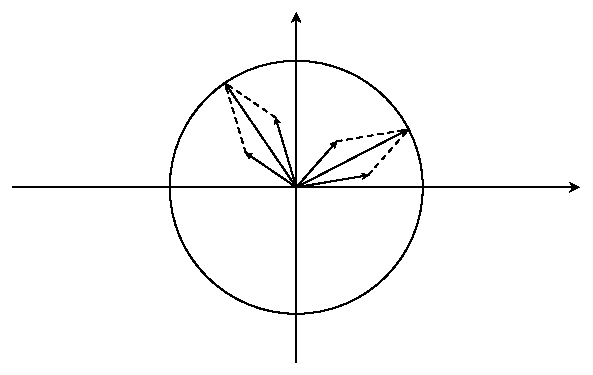
\includegraphics{Images/Rotazione.pdf}
\end{center}
La rotazione attorno all'origine è lineare in quanto ruotare due vettori e farne la somma equivale a fare la somma dei due per poi ruotarla. Formalmente:
\[
	rot\left( v_1+v_2 \right) = rot\left( v_1 \right)  + rot\left( v_2 \right)
\]
ossia la funzione $ rot $ è lineare e può quindi essere espressa tramite matrice associata
\begin{itemize}
	\item Uso base canonica di $ \R^{2} $, ossia i vettori $ \left( 1,0 \right) , \left( 0,1 \right)  $
	\item Calcolo $ rot\left( \left( 1,0 \right)  \right)  $ e $ rot\left( \left( 0,1 \right)  \right)  $
	\item Visto che la base scelta per il dominio coincide con quella del codominio posso mettere direttamente i vettori ottenuti come colonne della matrice, ottenendo:
	      \[
		      R_{\theta }=\begin{bmatrix}
			      \cos \theta & - \sin \theta \\
			      \sin \theta & \cos \theta
		      \end{bmatrix}
	      \]
\end{itemize}
\subsubsection*{Traslazione}
\begin{center}
	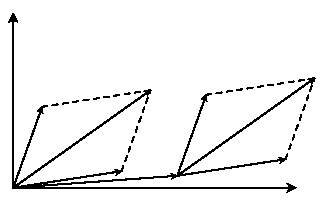
\includegraphics{Images/Traslazione.pdf}
\end{center}
La traslazione \underline{non} è una funzione lineare! Non vale
\[
	tr\left( v_1+v_2 \right) = tr\left( v_1 \right)  + tr\left( v_2 \right)
\]
e nemmeno
\[
	tr\left( kv_1 \right) = k\cdot tr\left( v_1 \right)
\]
(occhio a non farti fottere dalla traslazione del vettore geometrico, la somma di 2-uple va interpretata come somma di vettori dall'origine alla coordinata indicata, non tramite la regola del parallelogramma)
\subsubsection*{Speculare rispetto ad una retta}
\begin{center}
	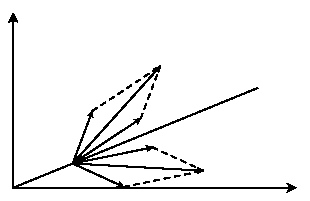
\includegraphics{Images/Speculare.pdf}
\end{center}
In questo caso possiamo notare che la trasformazione è lineare e quindi vale che
\[
	rif\left( v_1+v_2 \right) = rif\left( v_1 \right) + rif \left( v_2 \right)
\]
e anche che
\[
	rif\left( kv_1 \right) = k rif\left( v_1 \right)
\]
Per elaborare la matrice associata alla trasformazione possiamo scegliere una base opportuna, più comoda rispetto alla base canonica
\begin{itemize}
	\item Scelgo la base che ha come "assi cartesiani" la retta coincidente a quella secondo cui speccchiare e una retta perpendicolare a questa passante per l'origine.
	\item Secondo questa base $ \mathcal{B} = \left\{ u_1,u_2 \right\}  $posso calcolare facilmente il vettore simmetrico
	      \begin{itemize}
		      \item $ T\left( u_1 \right) = u_1  $
		      \item $ T\left( u_2 \right) = T\left( \left( 0,1 \right)  \right)  = \left( 0,-1 \right) $
	      \end{itemize}
\end{itemize}
quindi la matrice associata è:
\[
	\begin{bmatrix}
		1 & 0  \\
		0 & -1
	\end{bmatrix}
\]

\section{Autovalori e autovettori}
Partiamo osservando che se ho una matrice diagonale ()
\begin{definizione}{Autovalore e autovettore}
	Sia $ A \quad n \times n $. Un vettore \underline{non nullo} $ x \in  \mathbb{K}^{n} $ è detto \underline{autovettore} di $ A $ se esiste uno scalare $ \lambda \in \mathbb{K} $ tale che
	\[
		Ax = \lambda  x
	\]
	$ \lambda  $ è detto \underline{autovalore} di $ A $ associato a $ x $
\end{definizione}
Lo stesso ragionamento può essere esteso a qualsiasi funzione lineare
\vskip3mm
Gli autovettori sono una figata in quanto "eistono" in natura (se una matrice rappresenta un fenomeno fisico, gli autovettori hanno significato). Ad esempio in una matrice degli sforzi gli autovettori rappresentano i punti di maggiore tensione

\begin{teorema}{Matrice diagonale autovettori}
	Sia $ T : V \to V $ un endomorfismo. Allora:
	\begin{center}
		$ T $ ha una matrice diagonale associata $ \Leftrightarrow $ $ V $ ha una base associata formata da autovettori di $ T $
	\end{center}
\end{teorema}
\label{teo:diagonalizzabilità}
Dimostrazione $ \Leftarrow $. Se ho una base formata da autovettori allora esiste una matrice diagonale associata
\begin{itemize}
	\item Sia $ \mathcal{B}= \left\{ u_1,\ldots,u_n \right\}  $ una base di \underline{autovettori}
	\item Creo la matrice associata, calcolando $ T\left( u_i \right)  $ e mettendo il risultato come colonna di $ M_{ \mathcal{B}} \left( T \right)  $
	\item Considero che $ T\left( u_j \right) = \lambda_j u_j $ in quanto $ u_j $ è autovettore. Le sue coordinate rispetto alla base $ \mathcal{B} $ saranno $ \left( 0,\ldots, \lambda_1, \ldots, 0 \right)  $ con $ \lambda_1 $ in posizione $ j $
	\item Costruendo una matrice con questi vettori ottengo chiaramente una \underline{matrice diagonale}
\end{itemize}
Dimostrazione $ \Rightarrow $. Se esiste una matrice diagonale associata allora esiste una base composta da autovettori
\begin{itemize}
	\item Sia $ \mathcal{B} = \left\{ u_1,\ldots,u_n \right\}  $ una base di $ V $
	\item Come sappiamo la matrice associata è costruita mettendo come colonne gli elementi $ T\left( u_1 \right) ,\ldots, T\left( u_n \right)  $
	\item Se la matrice è diagonale, questa avrà forma
	      \[
		      \begin{bmatrix}
			      \lambda 1 & 0          & \ldots & 0          \\
			      0         & \lambda  2 & \ldots & \vdots     \\
			      \vdots    & \vdots     & \ddots & \vdots     \\
			      0         & 0          & \ldots & \lambda _n
		      \end{bmatrix}
	      \]
	      significa che il primo elemento di $ \mathcal{B} $ avrà coordinate $ \left( \lambda _1,0,\ldots,0 \right)  $ secondo $ \mathcal{B} $. Più in generale $ T\left( v_i \right)  $ ha coordinate $ \left( 0,\ldots, \lambda _i, \ldots,0 \right)  $ secondo $ \mathcal{B} $
	\item Ciò significa che $ T\left( v_i \right) = 0 v_1 + \ldots + \lambda_1 v_i + \ldots+ 0 v_n =\lambda _1 v_i$ ossia che $ v_i $ è un \underline{autovettore} (per ogni $ i $)
\end{itemize}

\begin{definizione}{Diagonalizzabilità}
	$ T $ si dice \underline{diagonalizzabile} se esiste una matrice associata diagonale:
	\[
		\exists M_B \left( T \right) \text{ diagonale }
	\]
\end{definizione}
NB: questo equivale a dire che $ M_{ \mathcal{B}}(T) $ è diagonalizzabile se esiste una matrice simile diagonale, ossia:
\[
	D = P M_{ \mathcal{B}}\left( T \right) P^{-1}
\]
NB: se $ A = M_{ \mathcal{B}}\left( T \right) $ è diagonalizzabile, con $ D $ la sua matrice simile diagonale, allora $ A^{K} $ è simile a $ D^{k} $ in quanto:
\[
	A^{k}= \left( P A P^{-1} \right) ^{k} = \left( P D P^{-1} \right)\ldots \left( P D P^{-1} \right)
\]
essendo il prodotto matriciale associativo, tutte le $ PP^{-1} $ in mezzo si eliminano e ottengo che
\[
	A^{k}= P D^{k}P^{-1}
\]
\subsection{Autospazio}
\begin{definizione}{Autospazio}
	Sia $ T : V \to V $ un endomorfismo. Si dice \underline{autospazio} di $ T $ relativo all'autovalore $ \lambda  $ lo spazio vettoriale:
	\[
		E\left( \lambda  \right) = N\left( T- \lambda I_{n} \right) = \left\{ v \in  V| T\left( v \right) = \lambda  v \right\}
	\]
	ossia l'insieme degli autovettori di $ V $ più il vettore nullo (sempre presente)
\end{definizione}
NB: il medesimo discorso può essere fatto per una matrice associata ad una funzione lineare.
\subsubsection*{Determinare se un $ \lambda  $ è autovalore}
Noto che se $ T : V \to V $ è un endomorfismo di uno spazio $ n $ dimensionale posso identificare l'insieme dei suoi autovettori tramite un sistema lineare:
\[
	T\left( v \right) = \lambda  v \Leftrightarrow A x = \lambda x
\]
dove $ x= T_{ \mathcal{B}}\left( v \right)  $. Posso visualizzare l'esempio in $ \R^{2} $, come in figura seguente. In tale figura viene rappresentato come, presa qualsiasi base, costituita da qualsiasi vettore, valga sempre la relazione:
\[
	2v= 2 x + 2y = 2 \vec{u} + 2 \vec{w}
\]
Quindi se applico la funzione $ T $ su $ \vec{V}  $, è come applicare la funzione $M_{ \mathcal{B}  }\left( T \right) $ sulle coordinate di $ \vec{v}  $: se duplico un vettore è come duplicare le sue coordinate rispetto ad una base fissata
\begin{center}
	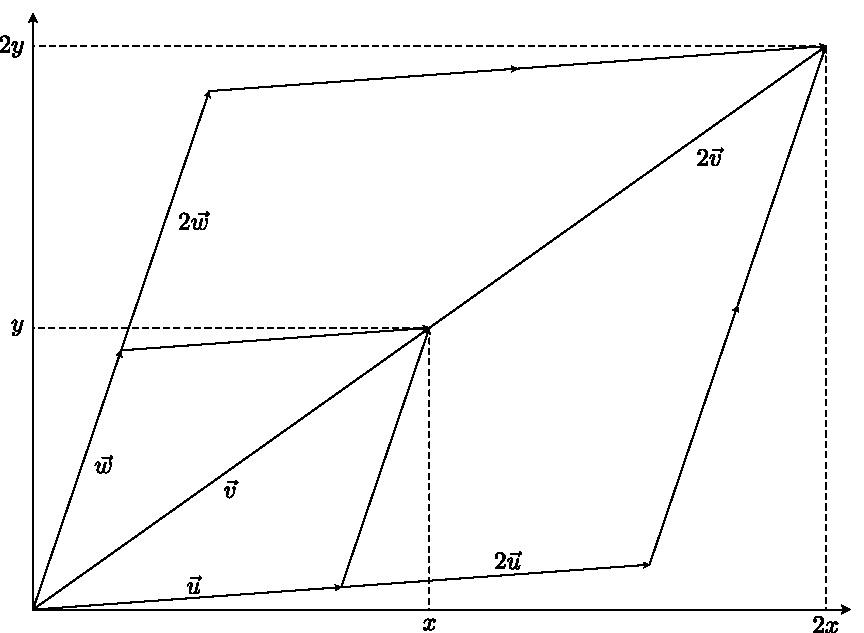
\includegraphics{Images/DetAutovalore.pdf}
\end{center}
quindi riprendendo la relazione espressa pocanzi, ossia che
\[
	T\left( v \right)  = \lambda v \Leftrightarrow Ax = \lambda x
\]
posso riportare il problema di trovare gli autovettori di una funzione alla risoluzione di un sistema omogeneo:
\[
	\left( A- \lambda  I_n \right) =0
\]
in quanto
\begin{itemize}
	\item $ \left( A- \lambda  I_n \right) x = ax - \lambda I_nx $ in quanto prodotto matriciale è distributivo
	\item $  ax - \lambda I_nx = Ax - \lambda x =0 \rightarrow Ax = \lambda  x$
\end{itemize}
\vskip3mm
NB: per trovare gli autovalori di una funzione lineare potrei studiare il sistema $ Ax = \lambda  x $, però risulterebbe più scomodo e difficile da gestire, perchè avrei un parametro sull'ultima colonna. Allora conviene lavorare sulla matrice $ Ax-\lambda I_n $, che la la seguente forma:
\[
	\begin{bmatrix}
		a_{11}-\lambda & \ldots & a_{1n}         \\
		\vdots         & \ddots & \vdots         \\
		a_{n1}         & \ldots & a_{nn}-\lambda \\
	\end{bmatrix}
\]
\subsection{Polinomi caratteristici}
\begin{definizione}{Polinomio caratteristico}
	Sia $ A $ una matrice $ n \times n $ e $ \lambda  $ un autovalore. Il polinomio di grado $ n $ nella variabile $ \lambda  $ è detto \underline{polinomio caratteristico} della matrice e si denota con:
	\[
		p_A\left( \lambda  \right) = \det \left( A- \lambda I_n \right)
	\]
	lo stesso discorso può essere fatto anche per un qualsiasi \underline{endomorfismo} $ T $
\end{definizione}
\begin{teorema}{Caratteristiche matrice $ Ax - \lambda  I_n $}
	\begin{itemize}
		\item Proprietà 1: uno scalare $ \lambda_0  $ è \underline{autovalore} di $ A $ se $ \lambda_0 $ è radice del polinomio caratteristico $ p_A \left( \lambda  \right)  $
		\item Proprietà 2: l'autospazio $ E\left( \lambda _0 \right)  $ ha dimensione $ n- rg \left( A- \lambda _0 I_n \right)  $
	\end{itemize}
\end{teorema}
Dimostrazione:
\begin{itemize}
	\item Proprietà 1:
	      \begin{itemize}
		      \item Se $ \lambda_0 $ è radice del polinomio caratteristico allora il determinante della matrice $ Ax - \lambda_0 I_n $ in corrispondenza di quel valore è \underline{nullo}
		      \item Se il determinante è nullo, il sistema omogeneo associato alla matrice ha \underline{infinite soluzioni}
		      \item Se il sistema $ \left( Ax - \lambda_0 x \right) = 0  $ ha soluzioni diverse dal vettore nullo significa che esistono autovettori con autovalore $ \lambda_0 $
	      \end{itemize}
	\item Proprietà 2:
	      \begin{itemize}
		      \item La dimensione dell'autospazio di $ A $ è uguale alla nullità del sistema lineare $ Ax - \lambda_0 I_n $ che identifica l'insieme degli autovettori
		      \item La nullità di tale sistema è uguale a $ n-rg\left( A- \lambda_0 I_n \right)  $
	      \end{itemize}
\end{itemize}
\begin{definizione}{Molteplicità algebrica}
	Data una matrice $ A $ si dice \underline{molteplicità algebrica} la molteplicità della radice $ \lambda_0 $ all'interno del polinomio caratteristico
\end{definizione}
\begin{definizione}{Molteplicità geometrica}
	Data una matrice $ A $ si dice \underline{molteplicità geometrica} la dimensione dell'autospazio $ E\left( \lambda_0 \right)  $:
	\[
		m_{geo}\left( \lambda_0 \right) = n - rg \left( A- \lambda_0 I_n \right)
	\]
	si può dimostrare che la molteplicità algebrica di un $ \lambda_0 $ nel polinomio caratteristico è sempre $ \ge $ alla molteplicità geometrica
	\[
		m_{alg}\left( \lambda_0 \right) \ge m_{geo}\left( \lambda_0 \right) \ge 1
	\]
\end{definizione}
\subsubsection*{Esempio 1}
La matrice reale $ A= \begin{bmatrix}
		0  & -3 & -1 \\
		6  & 11 & 3  \\
		10 & 15 & 7
	\end{bmatrix} $ ha polinomio caratteristico
\[
	p_A(\lambda)= \det
	\begin{bmatrix}
		-\lambda & -3         & -1        \\
		6        & 11-\lambda & 3         \\
		10       & 15         & 7-\lambda
	\end{bmatrix}
	= \det
	\begin{bmatrix}
		-\lambda & 0           & -1        \\
		6        & 2-\lambda   & 3         \\
		10       & 3 \lambda-6 & 7-\lambda
	\end{bmatrix}
\]

\[
	=(2-\lambda) \det
	\begin{bmatrix}
		-\lambda & 0  & -1        \\
		6        & 1  & 3         \\
		10       & -3 & 7-\lambda
	\end{bmatrix}
	=(2-\lambda)(-\lambda(16-\lambda)+28)=(2-\lambda)\left(\lambda^2-16 \lambda+28\right)
\]

\[
	=-(\lambda-2)^2(\lambda-14) .
\]
Dunque $A$ ha autovalori 2 e 14 , con autovettori rispettivamente
\[
	E(2)=N\left(A-2 I_3\right)=
	\begin{bmatrix}
		-2 & -3 & -1 \\
		6  & 9  & 3  \\
		10 & 15 & 5
	\end{bmatrix}
	=
	\begin{bmatrix}
		-2 & -3 & -1 \\
		0  & 0  & 0  \\
		0  & 0  & 0
	\end{bmatrix}
	=\left<\left( -\frac{3}{2}, 1, 0 \right) , \left( -\frac{1}{2},0,1 \right)  \right>
\]
nota che l'insieme generatore dell'insieme soluzione lo ho ricavato passando dalla matrice al sistema, per poi scriverlo in maniera parametrica, dando il valore $ t $ e $ s $ alle variabili libere:
\[
	-2x -3x -1 = 0 \rightarrow
	\begin{cases}
		x = -\frac{2}{3}s - \frac{t}{2} \\
		y = s                           \\
		z = t
	\end{cases}
\]
se leggi "in verticale" il sistema ti accorgi che è una combinazione lineare:
\[
	\left( -\frac{3}{2}, 1, 0 \right) s + \left( -\frac{1}{2}, 0, 1\right)t
\]
NB: in base alle variabile che scegli come variabili libere potresti ottenere vettori diversi, che però generano il medesimo sottospazio vettoriale. Per verificare che lo spazio generato coincida devi:
\begin{itemize}
	\item Creare una matrice che contenga tutti i vettori generatori come colonne
	\item Ridurre con Gauss-Jordan
	\item Verificare che la soluzione dipenda da almeno 2 variabili libere (nel nostro caso): ogni variabile libera corrisponde ad un coefficiente della combinazione lineare del vettore 3 e 4. Ciò significa che ogni vettore contenuto nel secondo sottospazio può essere ottenuto tramite combinazione linare dei primi due vettori
\end{itemize}
allo stesso modo per l'altro autovalore ottengo che:
\[
	E(14)=N\left(A-14 I_3\right)=N
	\begin{bmatrix}
		-14 & -3 & -1 \\
		6   & -3 & 3  \\
		10  & 15 & -7
	\end{bmatrix}
	=
	\begin{bmatrix}
		1 & 0 & 1 / 5  \\
		0 & 1 & -3 / 5 \\
		0 & 0 & 0
	\end{bmatrix}
	= \left( -\frac{1}{5}, - \frac{3}{5}, 1 \right) = \left( -1,3,5 \right)
\]

Le molteplicità algebriche e geometriche coincidono per i due autovalori. La matrice è diagonalizzabile, poiché l'insieme di autovettori
\[
	\mathcal{B}=\{(1,0,-2),(0,1,-3),(1,-3,-5)\}
\]
forma una base di $\mathbb{R}^3$, rispetto alla quale l'endomorfismo definito da $A$ ha matrice associata diagonale (nota che non serve che mi calcoli $ T\left( u_j \right)  $ per ogni elemento, visto che per il teorema \textit{teorema  \ref{teo:diagonalizzabilità}} so già che se ho una base di autovettori allora esiste una matrice diagonale associata con le $ \lambda  $ lungo la diagonale)
\[
	D=M_{\mathcal{B}}\left(T_A\right)=\left[\begin{array}{ccc}
			2 & 0 & 0  \\
			0 & 2 & 0  \\
			0 & 0 & 14
		\end{array}\right]
\]

Posso verificare costruendo la matrice associata alla funzione $ T $ secondo la base $ \mathcal{B} $:
\[
	M_{ \mathcal{B}}^{ \mathcal{E} }\left( T_A \right)=
	\begin{bmatrix}
		2  & 0  & 14  \\
		0  & 2  & -42 \\
		-4 & -6 & -70 \\
	\end{bmatrix}
\]
\begin{teorema}{Indipendenza autovettori}
	Se prendiamo $ n $ autovettori $ v_1,\ldots,v_{n} $ relativi a $ n $ autovalori distinti $ \lambda_1,\ldots, \lambda_n $ essi sono linearmente indipendenti.
\end{teorema}
\label{teo:indipendenzaAutovettori}
\textbf{Dimostrazione}: supponiamo di avere solo 2 autospazi
\begin{itemize}
	\item Supponiamo per assurdo che l'unione degli autospazi $ A $ e $ B $ sia \underline{linearmente dipendente}
	\item Ciò significa che almeno un autovettore di questo insieme può essere ottenuto come combinazione lineare di altri autovettori
	\item Otterrei quindi un autovettore $ v $ dell'insieme $ A $ come combinazione lineare degli elementi dell'insieme $ B $ (o viceversa)
	\item Ciò tuttavia è assurdo: visto che l'autovettore $ v \in A	$ è relativo all'autovalore $ \lambda_a $. Tuttavia questo appartiene all'insieme $ B $. L'unica soluzione è quindi che $ \lambda_a $ e $ \lambda_b $ siano uguali
\end{itemize}

\begin{teorema}{Unione di autospazi}
	L'unione di basi di autospazi distinti è un insieme \underline{linearmente indipendente}
\end{teorema}
\label{teo:unioneAutospazi}
\textbf{Dimostrazione}:
\begin{itemize}
	\item Autovettori relativi ad autovalori differenti sono \underline{linearmente indipendenti} (vedi \textit{teorema  \ref{teo:indipendenzaAutovettori}})
	\item Gli autovettori che costituiscono la base di un autospazio sono necessariamente \underline{linearmente indipendenti}
	\item Ho insiemi di elemti linearmente indipendenti in cui ogni elemento è linearmente indipendente con ogni altro elementi di ogni altro insieme. Per questo l'insieme è tutto \underline{linearmente indipendente}
\end{itemize}
\begin{teorema}{Teorema di diagonalizabilità}
	Sia $ T: V \to V $ un endomorfismo. Siano $ \lambda_1,\ldots, \lambda_h $ gli autovalori distinti di $ T $. Allora
	\[
		T  \text{ è \underline{diagonalizzabile} } \Leftrightarrow \sum_{i=1}^{h} m_{geo}\left( \lambda_i \right) = \sum_{i=1}^{h} \dim E \left( \lambda_i \right) =n = \dim V
	\]
\end{teorema}
\textbf{Dimostrazione} $ \Rightarrow $ : se $ T $ è diagonalizzabile $ \Rightarrow $ la somma delle molteplicità geometriche è uguale a $ \dim V $
\begin{itemize}
	\item  Se un endomorfismo è diagonalizzabile, secondo una data base $ \mathcal{B} $ la sua matrice associata e la sua matrice $ A - I_n \lambda  $ avranno rispettivamente forma:
	      \[
		      \begin{bmatrix}
			      \lambda_1 & 0         & 0         & 0      \\
			      0         & \lambda_1 & 0         & 0      \\
			      0         & 0         & \lambda_2 & 0      \\
			      0         & 0         & 0         & \ddots \\
		      \end{bmatrix}
		      \quad
		      \rightarrow
		      \quad
		      \begin{bmatrix}
			      \lambda_1-\lambda & 0                  & 0                   & 0      \\
			      0                 & \lambda_1 -\lambda & 0                   & 0      \\
			      0                 & 0                  & \lambda_2 - \lambda & 0      \\
			      0                 & 0                  & 0                   & \ddots \\
		      \end{bmatrix}
	      \]
	\item Quindi il polinomio caratteristico avrà forma $ \left( \lambda_1 - \lambda  \right)^{m_{\lambda_1}} \ldots \left( \lambda_n - \lambda  \right)^{m_{\lambda_m}}$ dove $ m_{\lambda_m} $ è la molteplicità algebrica dell'autovalore $ \lambda_m $
	\item La somma delle \underline{molteplicità algebrica} è quindi $ n = \dim  V $
	\item Stessa cosa vale per le \underline{molteplicità geometriche}: in corrisponsenza di un autovalore $ \lambda_m $ con molteplicità $ m_{\lambda_m} $ otterrò un sistema con $ m $ righe nulle. La sua nullità, ossia la dimensione di $ E\left( \lambda_m \right)=m_{\lambda_m}  $. La somma delle nullità è $ n = \dim  V $
\end{itemize}
\textbf{Dimostrazione} $ \Leftarrow $: la somma delle molteplicità geometriche e algebriche è uguale a $ \dim V  \Rightarrow  T $ è diagonalizzabile
\begin{itemize}
	\item Se la somma delle \underline{molteplicità geometriche} è uguale a $ n = \dim V $ so di avere $ n $ autovettori che per il \textit{teorema  \ref{teo:unioneAutospazi}} sono tutti \underline{linearmente indipendenti}
	\item Essendo tutti gli $ n $ vettori linearmente indipendenti, questi formano una base. Per \textit{teorema  \ref{teo:diagonalizzabilità}}
\end{itemize}
NB: se il polinomio caratteristico ha tutte le sue radici nel campo $ \mathbb{K} $ allora è sufficiente controllare che in corrispondenza di ogni autovalore $ \lambda_m $ la molteplicità geometrica e algebrica coincidano:
\[
	m_{alg}\left( \lambda_i \right) = m_{geo}\left( \lambda_i \right) \quad \forall i = 1, \ldots, m
\]
\section{Basi ortonormali e teorema spettrale}
Quando si studiano problemi che riguardano lunghezze di vettori, ortogonalità o angoli è comodo utilizzare delle basi di tipo particolare

\begin{definizione}{Base ortonormale}
	Una base $ \mathcal{B}= \left\{ u_1,\ldots,u_m \right\}  $ di un sottospazio $ U $ di $ \R^{n} $ è una \underline{base ortonormale} di $ U $ se
	\[
		u_i \cdot u_j = 0 \text{ per } i \neq j \quad \text{ e } \quad  u_i \cdot u_j = 1 \text{ per } i=1,\ldots,m
	\]
\end{definizione}

NB: le basi canoniche di $ \R^{n} $ sono ortonormali
\vskip3mm
Vi è una proprietà importante:
\begin{tcolorbox}
	Se $\mathcal{B}=\left\{u_1, \ldots , u_m\right\}$ è una base ortonormale di $U$, le coordinate $x_1, \ldots, x_m$ di un vettore $v \in U$ rispetto a $\mathcal{B}$ si ottengono mediante il prodotto scalare

\end{tcolorbox}

\[
	x_j=v \cdot u_j, \quad j=1, \ldots, m .
\]
\textbf{Dimostrazione:}
\begin{itemize}
	\item Se $v=x_1 u_1+\cdots+x_m u_m$, allora $v \cdot u_j=\left( \sum_{i=1}^m x_iu_i \right)\cdot u_j$
	\item Posso portarte per le proprietà delle sommatorie $ u_j $ al suo interno: $ \sum_{i=1}^{m} \left( x_i u_i \right) \cdot u_j $
	\item Visto che il prodotto scalare è \underline{bilineare}, posso applicare la proprietà associativa $  \sum_{i=1}^{m}  x_i \left( u_i \cdot u_j \right) $
	\item Noto che per definizione di base ortogonale, il prodotto scalare $ \left( u_i \cdot u_j \right)  $ è 1 se $ i=j $, altrimenti 0. La sommatoria è quindi uguale a $ x_j $:
	      \[
		      \sum_{i=1}^{m} x_i \left( u_i \cdot u_j \right) = x_j
	      \]
\end{itemize}
\subsection{Costruzione basi ortonormali Gram-Schmidt}
A partire da una base $\left\{v_1, \ldots, v_m\right\}$ di $U$, si può costruire una base ortonormale di $U$. Si procede ricorsivamente, ponendo $u_1=\frac{v_1}{\left\|v_1\right\|}$ e poi definendo in successione i vettori $u_2, \ldots, u_m$ con la formula
con $c \in \mathbb{R}$ scelto in modo che sia $\left\|u_k\right\|=1$.
\[
	u_k=c\left(v_k-\sum_{i=1}^{k-1}\left(v_k \cdot u_i\right) u_i\right)
\]


\begin{center}
	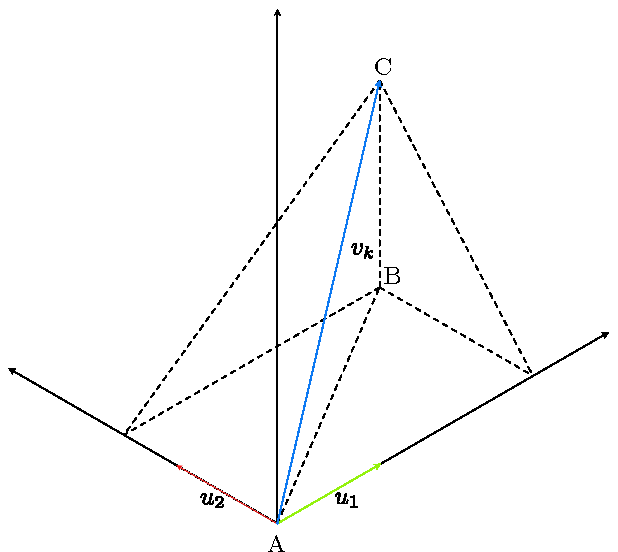
\includegraphics{Images/Gram scmidt.pdf}
\end{center}

Per farsi un'idea del funzionamento della formula di Gram Schmidt posso procedere fino ad $ \R^{3} $
\begin{itemize}
	\item L'idea è che \underline{la sommatoria} della formula crea un vettore che sottratto $ v_k $ ne crea uno ortogonale agli elementi della base ortonormale calcolati fino a quel momento
	\item Analiziamo la sommatoria
	      \[
		      \sum_{i=1}^{k-1}\left(v_k \cdot u_i\right) u_i
	      \]
	      sappiamo che il prodotto scalare è uguale a $ \|v_1\|\|v_2\| \cos \left( \theta  \right)  $
	\item La sommatoria diventa quindi:
	      \[
		      \sum_{i=1}^{k-1}\|v_k\| \|u_i\| \cos \left( \theta  \right)  u_i
	      \]
	      tuttavia, ricordiamo che per definizione ogni elemento della base ortonormale ha norma $ =1 $, quindi $ \|u_i\|=1 $ e la sommatoria diventa:
	      \[
		      \sum_{i=1}^{k-1}\|v_k\|  \cos \left( \theta  \right)  u_i
	      \]
	\item Visto che $ u_i $ ha norma $ 1 $, la quantà all'interno della sommatoria è la \underline{proiezione ortogonale} di $ v_k $ su $ u_i $
	\item Nota che la somma delle proiezioni ortogonali su ogni $ u_i $ danno creanno la proiezione ortogonale di $ v_k $ sul piano $ \left( \overline{AB} \right)  $. Se a $ v_k$ sottraggo tale proiezione ottengo $ \left( \overline{BC} \right)  $, il quale è chiaramente ortogonale sia a $ u_1 $ che $ u_2 $
\end{itemize}







Esempio. Dalla base $\mathcal{B}=\{(1,0,1),(1,0,0),(2,1,0)\}$ di $\mathbb{R}^3$, con il prodotto canonico, mediante il procedimento di Gram-Schmidt si ottiene

\[
	u_1=\frac{v_1}{\left\|v_1\right\|}=\frac{1}{\sqrt{2}}(1,0,1)=\left(\frac{1}{\sqrt{2}}, 0, \frac{1}{\sqrt{2}}\right)
\]
\[
	v_2-\left(v_2 \cdot u_1\right) u_1=(1,0,0)-\frac{1}{\sqrt{2}} \frac{1}{\sqrt{2}}(1,0,1)=\left(\frac{1}{2}, 0,-\frac{1}{2}\right)
\]
da cui
\[
	u_2=\frac{v_2-\left(v_2 \cdot u_1\right) u_1}{\left\|v_2-\left(v_2 \cdot u_1\right) u_1\right\|}=\sqrt{2}\left(\frac{1}{2}, 0,-\frac{1}{2}\right)=\left(\frac{1}{\sqrt{2}}, 0,-\frac{1}{\sqrt{2}}\right)
\]
\[
	v_3-\left(v_3 \cdot u_1\right) u_1-\left(v_3 \cdot u_2\right) u_2=(2,1,0)-\sqrt{2}\left(\frac{1}{\sqrt{2}}, 0, \frac{1}{\sqrt{2}}\right)-\sqrt{2}\left(\frac{1}{\sqrt{2}}, 0,-\frac{1}{\sqrt{2}}\right)=(0,1,0)
\]
da cui
\[
	u_3=(0,1,0)
\]
quindi
\[
	u_1 = \left( \frac{1}{\sqrt{2} },0, \frac{1}{\sqrt{2} } \right) \quad u_2= \left( \frac{1}{\sqrt{2} },0,-\frac{1}{\sqrt{2} } \right) \quad  u_3= \left( 0,1,0 \right)
\]
Nota che la matrice di transizione $ M_{ \mathcal{B}}^{ \mathcal{E}} \left( Id \right)  $ ha come colonne i vettori della base ortonormale. Quindi, indicando con $ P^{i} $ e $ P^{j} $ rispettivamente la $ i $ esima e la $ j $ esima colonna ho che:
\[
	P^{i}\cdot P^{j}=
	\begin{cases}
		1 \text{ per }i = j \\
		0 \text{ pet }i \neq j
	\end{cases}
	\quad \text{ ossia } \quad
	P^{T} P = I_n
\]
da questa caratteristica si ricava la definizione di \underline{matrice ortogonale}

\begin{definizione}{Matrice ortogonale}
	Una matrice quadrata $ P \in  M_n \left( \R \right)  $ è detta \underline{ortogonale} se $ P^{-T} P = I_n $
\end{definizione}

\begin{teorema}{Prerequisito 1 teorema spettrale}
	Sia $ A $ una matrice reale \underline{simemtrica} $ n \times n $. Allora $ A $ ha $ n $ autovalori reali, contati con la loro \underline{molteplicità algebrica}
\end{teorema}
Nota che
\label{teo:prerequisitoSpettrale}
\textbf{Dimostrazione}: l'idea generale è quella di ottenere due identità, e confrontarle a loro volta
\vskip3mm
Sia $ T_A:\C ^{n} \to C^{n} $ l'endomorfismo definito da $ A $. Sia $  c \in \C^{n}, x \neq 0 $ un autovettore di $  T_A $ con autovaloce $ \lambda  \in \C $

\begin{itemize}
	\item \textbf{Itendità 1}: se $ x $ è autovettore relativo a $ \lambda  $ allora:  $ Ax = \lambda x$
	      \begin{itemize}
		      \item Posso applicare la funzione "trasposta" ad ambo i membri, ottenendo:
		            \[
			            x^{T} A = \lambda  x^{T}
		            \]
		            nota bene che nel membro sinistro $ x $ e $ A $ si scambiano per via delle proprietà delle matrici trasposte
		      \item Posso applicare la funzione "negato" (negato di un numero complesso) ad ambo i membri, ottenendo:
		            \[
			            \bar{x}^T A = \bar{\lambda} \bar{x}^T
		            \]
		            \begin{itemize}
			            \item A sinistra $ A = \overline{A} $ in quanto la matrice $ A $ è a \underline{coefficienti reali}
			            \item A destra posso affermare che $ \overline{\lambda  x ^{T}} = \overline{\lambda }\overline{x}^{T} $ in quanto la funzione "negato" è \underline{lineare}(se ci pensi è una riflessione rispetto all'asse $ x $)
		            \end{itemize}
		      \item Moltiplicando a destra e a sinistra per $ x $ ottengo:
		            \begin{equation*}
			            \overline{x}^{T}Ax = \overline{\lambda }\overline{x}^{T}x
		            \end{equation*}
	      \end{itemize}
	\item \textbf{Identità 2:} parto sempre dall'identità  $ Ax = \lambda x $
	      \begin{itemize}
		      \item Moltiplico a destra e a sinistra per $ x^{-T} $ e ottengo:
		            \[
			            \overline{x}^{T}Ax = \overline{x}^{T}\lambda x
		            \]
		      \item Nel termine di destra, posso spostare lambda in quanto è solo un coefficiente, ottenendo:
		            \begin{equation*}
			            \overline{x}^{T}Ax = \lambda \overline{x}^{T} x
		            \end{equation*}
	      \end{itemize}
	\item \textbf{Metto assieme} tramite il termine di sinistra l'identità 1 e 2 ottengo che :
	      \[
		      \overline{\lambda }\overline{x}^{T}x = \lambda \overline{x}^{T}x
	      \]
	      quindi necessariamente $ \overline{\lambda } = \lambda  $ ossia $ \lambda  $ è un numero \underline{reale}!
\end{itemize}
Nota bene che l'identità non può essere soddisfatta imponenendo $ \overline{x}^{T}x =0$ in quanto questa quantità è sempre $ \ge 0 $:
\[
	\overline{x}^{T}x =
	\begin{bmatrix}
		\overline{x_1} \\
		\overline{x_2} \\
		\vdots         \\
		\overline{x_n}
	\end{bmatrix}
	\begin{bmatrix}
		x_1 & x_1 & \ldots & x_n
	\end{bmatrix}
	=
	\overline{x_1}x_1 + \overline{x_2}x_2 + \ldots + \overline{x_n}x_n
\]
il prodotto di un numero complesso con il suo coniugato è sempre diverso da 0 se $ z \neq 0 $:
\[
	z \overline{z} = c e^{\theta } c e^{-\theta } = c
\]
quindi visto che per ipotesi $ x \neq 0 $ anche la quantità $ \overline{x}^{T}x \neq 0$

\begin{teorema}{Teorema spettrale}
	Sia $ A  $ una matrice reale simmetrica $ n\times n $. Allora
	\[
		A \text{ è \underline{diagonalizzabile}}
	\]
	Esiste una base \underline{ortonormale} di $ \R^{n} $costituita da autovettori di $ A $, cioè esiste una matrice ortogonale di $ P $ tale che $ P^{-1}A P = D$ sia \underline{diagonale}
\end{teorema}
\textbf{Dimostrazione}: la dimostrazione procede per induzione
\begin{itemize}
	\item Caso base: se $ n = 1 $ chiaramente l'ipotesi è verificata. Qualsiasi base costituita da un vettore con norma 1 costituisce una base ortonormale
	\item Ora devo dimostrare che se l'ipotesi è vera per $ n-1 $ allora lo è necessariamente anche per $ n $
	\item Visto che $ A $ è simmetrica per ipotesi, per il \textit{teorema \ref{teo:prerequisitoSpettrale}} ho almeno un autovalore \underline{reale} $ \lambda_1 $ di $ A $. L'autovettore $ u_1 $ corrispondente a $ \lambda_1 $ costituirà il primo elemento della base di $ \R^{n} $
	\item Ora considero lo spazio vettoriale $ U^{\perp} $ indivituato dai vettori ortogonali a $ u_1 $. Questo spazio ha dimensione $ n-m $, dove $ m $ è la dimensione del sottospazio a cui è ortogonale $ U^{\perp} $. Nel nostro caso, il sottospazio è individuato dai vettori $ \perp $ a $ u_1 $. Visto che il sottospazio generato da $ u_1 $ è 1, allora la  $ \dim U^{\perp} = n-1$
	\item Noto che $ Av \in U^{\perp} $ per ogni $ v \in U^{\perp} $
	      \[
		      (A v) \cdot u_1=(A v)^T u_1=\left(v^T A^T\right) u_1=v^T\left(A u_1\right)=v^T\left(\lambda_1 u_1\right)=\lambda_1\left(v \cdot u_1\right)=0
	      \]
	      \[
		      \left( Av \right) \cdot u_1 = 0 \rightarrow Av \perp u_1
	      \]
	\item Ciò vuol dire che posso condierare $T_A : U^{\perp} \to U^{\perp} $ anzichè $ T_A : \R^{n} \to \R^{n} $
	\item Se ora suppongo induttivamente che $T_A : U^{\perp} \to U^{\perp} $ abbia una base ortonormale, necessariamente anche $ T_A \R^{n} \to \R^{n} $ avrà una base ortonormale, costituita dal vettore $ u_1 $ e dagli $ n-1 $ vettori che costituiscono la base di $ U^{\perp} $
	\item Ho finito la dimostrazione: se la tesi vale per $ n-1 $ allora vale anche per $ n $. Visto che è vera per $ n=1 $, allora deve essere vera per ogni $ n $
\end{itemize}
NB: se una matrice $ A $ è simmetrica, so per certo che \underline{vettori appartenenti ad autospazi relativi ad autovalori differenti, sono sempre ortogonali}

\end{document}
